\documentclass[a4paper, 10pt, oneside, titlepage, openany, onecolumn, final]{book}

\usepackage{style}

\title{\tb{Topología Elemental}}
\author{Álvaro García Tenorio \and Manuel Navarro García\and Iván Prada Cazalla \and Álvaro Rodríguez García \and Clara Rodríguez Núñez}
\date{\today}

\begin{document}
	%Título e Índice
	\maketitle
	\tableofcontents
		
	%Capítulos
	%Investigar para que el prefacio sea un capítulo distinguido.
	%Para este capítulo se usará la abreviatura "pref"
\section*{Prefacio}
%No se hasta que punto es recomendable referenciar el prefacio siendo la chapuza que es.
\label{pref}
Estas notas son una transcripción de las clases de la asignatura ``\ti{Topología Elemental}'', impartidas por Jesús María Ruiz Sancho en el curso 2016--2017 a los cursos de tercero de los Dobles Grados de Matemáticas e Informática y Matemáticas y Física en la facultad de Ciencias Matemáticas de la Universidad Complutense de Madrid (UCM).

\subsection*{Agradecimientos}
En primer lugar hay que agradecer a todos aquellos que han estado pendientes de la evolución del texto durante su proceso de construcción, corrigiendo numerosas faltas de estilo y erratas de toda la clase y condición. Entre ellos queremos destacar a María José Belda Beneyto y Clara Isabel López González.

Por otra parte, en términos de dominio de \LaTeX\ y otras diversas herramientas que han mejorado mucho este texto destacamos especialmente a uno de los autores, Álvaro Rodríguez García.
	%Capítulos.
	
	\part{Topología general}	
	%---CAPITULO DOCUMENTADO CON PAUTAS Y PIJOTERÍAS DE ESTILO

%Generalidades:
%--Usar los entornos predefinidos en el style para teoremas y demás.
%--Cuanto más cosas se etiqueten mejor.
%--Nunca usar \\ para saltar de línea, en su lugar, dar a ENTER dos veces.
%--Redactar.
%Cuidado al usar interiores pues es algo que lamentablemente jode el interlineado. Usar el comando reducido \inter cuando se quiera poner un abierto en medio del texto.

%Para este capítulo se usará la abreviatura "etop".
\chapter{Espacios Topológicos}
%Todo capítulo será etiquetado con una abreviatura especificada al inicio del archivo.
\label{etop}
%Todo capítulo comienza con una breve introducción, ya sea a modo de breve motivación o a modo de resumen de contenidos (o ambas).
Al comienzo de este capítulo introducimos la noción de espacio topológico, introduciendo unos cuantos ejemplos, a continuación, presentaremos la dualidad entre conjuntos abiertos y cerrados.%Continuará.
\section{Espacios Topológicos. Definición y Ejemplos.}
%Etiquetaremos tanto secciones como subsecciones.
\label{etop_definicionEjemplos}
%Es recomendable redactar un poco entre entorno y entorno y soltar un chascarrillo de vez en cuando para dejar reflexionar al lector y que no le parezca un ladrillo.
Comenzamos, como no podía ser de otra manera, definiendo la estructura sobre la que trabajaremos a lo largo de todas estas notas, los llamados espacios topológicos.
%Es recomendable titular cada entorno entre corchetes.
\begin{defi}[Espacio Topológico]
	%Cada vez que comencemos un entorno potencialmente referenciable deberá ser etiquetado siguiendo un convenio similar a este.
	\label{etop_def_espacioTopologico}
	%Cada vez que introduzcamos un concepto nuevo es recomendable ponerlo en negrita y cursiva, se puede hacer usando estos comandos, probablemente haya que crear uno más corto porque la verdad que es un poco coñazo.
	Un \tbi{espacio topológico} es un conjunto arbitrario no vacío $\mc{X}$ equipado con una colección $\tau$ de subconjuntos $\mc{U}\subset\mc{X}$ que cumplen las siguientes propiedades
	%Cuando se está en un entorno es recomendable poner algo de texto antes de un enmerate para que quede mejor.
	\begin{enumerate}
		%Cuando se definen axiomas importantes en el enumerate se sustituyen los números por cosas que llaman la atención (se suele hacer muy pocas veces).
		\item[\tb{T1}] El vacío y el total están en la colección $\tau$, es decir, $\{\emptyset, \X\} \subset \tau$
		\item[\tb{T2}] La unión arbitraria de conjuntos de $\tau$ está en $\tau$. Escrito de forma más rigurosa, pero desde luego, menos elegante, 
		$\bigcup_{i\in I}\U_i\in\tau$ donde cada $\U_i\in\tau$.
		\item[\tb{T3}] La intersección finita de conjuntos de $\tau$ está en $\tau$. O, dicho de otra forma, $\bigcap_{i=1}^{n}\U_i\in\tau$ donde cada $\U_i\in\tau$.
	\end{enumerate}
\end{defi}
%Siempre viene bien algún chascarrillo para liberar tensiones.
Hagamos un par de pequeñas observaciones antes de continuar con nuestro recién empezado viaje cósmico--topológico.
\begin{obs}[Sutilezas]
	\label{etop_obs_sutilezas}
	Se desprende de la definición \ref{etop_def_espacioTopologico} que un espacio topológico no es más que un par $(\X, \tau)$. Como es natural, salvo que sea necesario, nos referiremos a un espacio topológico por el conjunto que lo conforma, al igual que hacemos en casi todas las ramas de las matemáticas (Espacios Vectoriales, Grupos, Anillos,...).
\end{obs}
Introducimos ahora un poco de terminología con la que el lector no tiene más remedio que hacerse familiar.
\begin{obs}[Terminología]
	\label{etop_obs_terminologia}
	A la familia de conjuntos $\tau$ que conforman un espacio topológico $\X$ se la denomina \tbi{topología} de $\X$.
	
	Asimismo, a los conjuntos que conforman $\tau$ reciben el nombre de \tbi{abiertos} de $\X$. Normalmente los denotaremos con las letras $\U$ o $\W$.
	
	Como es evidente, nos referiremos a los elementos de $\X$ como \tbi{puntos}.
\end{obs}
Introducimos ahora unos pocos ejemplos para irnos familiarizando con el concepto de espacio topológico. Viendo lo general que puede llegar a ser.
\begin{exa}[Topologías]
	\label{etop_exa_topologias}
	Las demostraciones de que, efectivamente, se cumplen las restricciones impuestas por la definición \ref{etop_def_espacioTopologico}, o bien ya se han hecho en cursos anteriores, o bien se dejan al lector como ejercicio inmediato.
	\begin{enumerate}
		\item El espacio ordinario $\R^n$ es un espacio topológico con la topología definida por los conjuntos abiertos en el sentido usual cuando hablamos de espacios métricos, es decir
		%Se pone una estrellita para que no introduzca número, si no ponemos la estrellita debemos etiquetar la ecuación.
		\begin{equation}
			\label{etop_eq_topologiaRn}
			\tau = \{\U\subset\R^n\tq \forall x\in\U\ \exists\  B(x,\varepsilon)\subset\U\}
		\end{equation}
		\item Una topología interesante por su simpleza, y por que dota a cualquier conjunto no vacío $\X$ con estructura de espacio topológico, es la llamada \tbi{topología trivial}, que viene definida por \begin{equation}
		\label{etop_eq_topologiaTrivial}
			\tau=\{\emptyset, \X\}
		\end{equation}
		\item Siguiendo la idea del ejemplo anterior, pero a la inversa, encontramos una topología que también toda de estructura topológica a cualquier conjunto no vacío $\X$. Esta topología viene dada por
		\begin{equation}
		\label{etop_eq_topologiaDiscreta}
			\tau = \partes(\X)
		\end{equation}
		A esta topología la llamaremos \tbi{topología discreta}.
		\item Como último ejemplo curioso nos queda la llamada \tbi{topología del punto}. Que consiste en considerar como abiertos a todos los subconjuntos de un conjunto $\X$ que contengan a un determinado punto $a$. Es decir
		\begin{equation}
		\label{etop_eq_topologiaPunto}
			\tau_a = \{\U \subset \X\tq a\in\U\}\cup\{\emptyset\}
		\end{equation}
		
		%Comento este ejemplo porque no se entiende un zipote lo que explicó este señor.
		
		%\item Como topología especial y rara, tomemos cuatro puntos a, b, c, d, siendo a y b cerrados, y c y d abiertos. Este espacio topológico es homótopo a la circunferencia $(S^{1})$ (viendo así que los conjuntos finitos pueden ser muy interesantes, aunque de primeras no nos lo imaginemos).
	\end{enumerate}
	Con lo que ya tenemos una gama lo suficientemente amplia de ejemplos como para ir tirando.
\end{exa}
En lo que resta de capítulo iremos introduciendo algunos conceptos generales de los que haremos uso de forma constante a lo largo del curso.
\section{Conjuntos Abiertos e Interior}
\label{etop_entornos}
En esta sección introducimos el concepto de entorno, cuya utilidad inmediata es caracterizar a los conjuntos abiertos de un espacio topológico $\X$.
\begin{defi}[Entorno de un Punto]
	\label{etop_def_entorno}
	Un \tbi{entorno} de un punto $a\in\X$ es un conjunto que contiene a un abierto que contiene al punto $a$.
\end{defi}
Normalmente denotaremos con la letra $\V$ a los entornos, esta costumbre se debe a un galicismo. %¿cuál?

Escribamos la definición de entorno \ref{etop_def_entorno} de forma conjuntista para que no quede ninguna duda
\begin{equation}
	\label{etop_eq_entorno}
	\V\supset\U\ni a
\end{equation}

Como ya adelantamos, se puede usar la noción de entorno para caracterizar a los abiertos, tal y como muestra el siguiente lema.
\begin{lem}[Caracterización de Abiertos]
	\label{etop_lem_caracterizacionAbiertos}
	$\U$ es abierto si y solo si es entorno de todos sus puntos.
\end{lem}
\begin{proof}
	Supongamos que $\U$ es abierto, entonces, dado un punto $a\in\U$ es evidente que $\U$ contiene a un abierto (él mismo) que contiene al punto $a$. Luego $\U$ es, trivialmente, entorno de todos sus puntos.
	
	Recíprocamente, si $\U$ es entorno de todos sus puntos, entonces, para cada punto $a\in\U$ se cumple que
	\begin{equation*}
		\U\supset\U_a\ni a
	\end{equation*}
	de donde se desprende que
	\begin{equation*}
		\U\supset\bigcup_{a\in\U}\U_a=:A
	\end{equation*}
	Más aún, se da la otra contención, y además, de forma trivial, ya que todo punto de $\U$ pertenece a algún $\U_a$, luego también a la unión de todos. Luego
	\begin{equation*}
		\U=A
	\end{equation*}
	Como la unión arbitraria de abiertos es abierto, $A$ es abierto, con lo que se sigue el resultado.
\end{proof}
En general, un conjunto será entorno de algunos de sus puntos, en principio no de todos. De esta idea surge la siguiente definición.
\begin{defi}[Punto Interior]
	\label{etop_def_puntoInterior}
	Dado un conjunto $A\subset\X$, diremos que un punto $a\in\X$ es un \tbi{punto interior} de $A$ si $A$ es entorno de $a$.
\end{defi}
Será algo habitual de ahora en adelante tratar de determinar el conjunto de puntos interiores de un determinado conjunto $A\subset\X$, a este conjunto se le denomina \tbi{interior} de $\X$.

Antes de continuar, fijemos unas cuantas notaciones que utilizaremos según el contexto para referirnos al interior de un conjunto.
\begin{equation}
\label{etop_eq_notacionInterior}
	\Int_{\X}(A)=\inter{A}=\Int(A)
\end{equation}
Antes de continuar, merece la pena notar que el interior de un conjunto puede ser el conjunto vacío, así como que trivialmente se da la desigualdad conjuntista
\begin{equation}
\label{etop_eq_desigualdadInterior1}
	\inter{A}\subset A
\end{equation}
Veamos ahora unos resultados elementales, pero a la vez cruciales del interior de un conjunto.
\begin{lem}[Apertura]
	\label{etop_lem_aperturaInterior}
	El interior de un conjunto $A$ es un abierto.
\end{lem}
\begin{proof}
	Para probar esto haremos uso del lema \ref{etop_lem_caracterizacionAbiertos}, es decir, trataremos de ver que es entorno de todos sus puntos.
	
	En efecto, dado un punto $a\in\inter{A}$, existe un abierto $\U_a\subset A$ de manera que $a\in\U_a$. Luego para ver que $\inter{A}$ es un entorno de $a$ basta demostrar la inclusión $\U_a\subset\inter{A}$, hagámoslo.
	
	Sea $x\in\U_a\subset A$, es claro que $A$ es entorno de $x$, luego $x\in\inter{A}$.
	
	Con lo cual hemos demostrado que $\inter{A}$ es entorno de todos sus puntos.
\end{proof}

El otro resultado elemental que caracteriza al interior de un conjunto $A$, es que es el mayor abierto contenido en $A$.

Presentamos aquí los primeros pasos de la demostración por ser especialmente útiles y omnipresentes en las matemáticas en general.

Como la unión de abiertos es abierto, es claro que una forma de construir el mayor abierto contenido en cierto conjunto es, coleccionar los abiertos contenidos en dicho conjunto y unirlos. Escrito formalmente, tomamos el conjunto
\begin{equation}
\label{etop_eq_mayorAbierto}
	B:=\bigcup_{\W\subset A}\W
\end{equation}
Es claro que $B\subset A$, ya que es una unión de conjuntos contenidos en $A$, además, si hubiera un abierto más grande contenido en $A$ que $B$, este pertenecería a la familia de conjuntos que estamos uniendo, lo cual es absurdo.

Presentamos el final de la demostración en forma de lema.
\begin{lem}[Caracterización del Interior]
	\label{etop_lem_caracterizacionInterior}
	El interior de un conjunto $A$ es el mayor abierto contenido en $A$.
\end{lem}
\begin{proof}
	Por el lema \ref{etop_lem_aperturaInterior} sabemos que $\inter{A}$ es abierto, luego, por la ecuación \eqref{etop_eq_mayorAbierto} solo queda probar la igualdad
	\begin{equation*}
		\inter{A}=\bigcup_{\W\subset A}\W\subset A
	\end{equation*}
	Y esto es prácticamente trivial, veámoslo.
	
	Por una parte, $\inter{A}$ es un abierto contenido en $A$, luego está contenido en la unión de los abiertos contenidos en $A$.
	
	Por otra parte, dado $x\in\bigcup_{\W\subset A}\W$, es claro que, como $\bigcup_{\W\subset A}\W\subset A$ es un abierto, $A$ es entorno de $x$, luego $x\in\inter{A}$, lo que concluye la demostración.
\end{proof}

El lema \ref{etop_lem_caracterizacionInterior} es bastante fuerte y produce algunos corolarios interesantes que presentamos a modo de observaciones.
\begin{obs}[Propiedades del Interior]
	\label{etop_obs_propiedadesInterior}
	Enumeramos algunas propiedades del interior.
	\begin{enumerate}
		\item El interior del interior de un conjunto es el interior de dicho conjunto. Si lo escribimos sin que suene como un trabalenguas tenemos
		\begin{equation}
		\label{etop_eq_dobleInterior}
			\inter{\inter{A}}=\inter{A}
		\end{equation}
		Esto es trivial ya que al ser $\inter{A}$ un abierto, el mayor abierto contenido en él es él mismo.
		\item Un abierto coincide con su interior, es decir
		\begin{equation}
			\label{etop_eq_abiertoInterior}
			A=\inter{A}
		\end{equation}
		Esto es cierto por la misma razón que lo es la ecuación \eqref{etop_eq_dobleInterior}.
		\item Los interiores preservan las contenciones. O lo que es lo mismo
		\begin{equation}
			\label{etop_eq_interiorContencion}
			A\subset B\ra \inter{A}\subset\inter{B}
		\end{equation}
		Esto es claro ya que, como $B$ contiene a $A$, el mayor abierto contenido en $B$ serán en general más grande que el mayor abierto contenido en cualquier subconjunto suyo.
	\end{enumerate}
	Esto ya nos da cierta artillería para defendernos con estos conjuntos.
\end{obs}
Con esto podemos decir que ya hemos liquidado todo lo referente a conjuntos abiertos.
\section{Conjuntos Cerrados y Adherencia}
\label{etop_cerradosAdherencia}
En esta sección estudiaremos los conjuntos cerrados.

Cabe destacar que la noción de ser cerrado no es exactamente la contraria a la de ser abierto, ya que, como veremos más adelante, hay conjuntos que no son ni abiertos ni cerrados así como conjuntos que son abiertos y cerrados a la vez.

\begin{defi}[Conjunto Cerrado]
	Un conjuto $\F$ de un espacio topológico $\X$ se dice \tbi{cerrado} si su complementario, $\X\setminus\F$, es abierto.
\end{defi}

Usualmente denotaremos a los conjuntos cerrados con las letras $\F$ o $\mc{H}$.

Usando propiedades básicas de teoría de conjuntos se obtienen algunas propiedades elementales de los conjuntos cerrados.
\begin{lem}[Propiedades de los Cerrados]
	\label{etop_lem_propiedadesCerrados}
	\begin{enumerate}
		\item El vacío y el total son cerrados.
		\item La intersección arbitraria de cerrados es cerrada.
		\item La unión finita de cerrados es cerrada.
	\end{enumerate}
\end{lem}
\begin{proof}Vayamos caso por caso.
	\begin{enumerate}
		\item $\X$ es cerrado pues $\X\setminus\X=\emptyset$ es abierto.
		
		Asimismo, $\emptyset$ es cerrado pues $\X\setminus\emptyset=\X$ es abierto.
		\item $\bigcap_{i\in I}\F_i$ es cerrado ya que
		\begin{equation*}
			\X\setminus\left(\bigcap_{i\in I}\F_i\right)=\bigcup_{i\in I}\X\setminus\F_i
		\end{equation*}
		es abierto por ser la unión arbitraria de abiertos un abierto.
		\item $\bigcup_{i=1}^n\F_i$ es cerrado, basta tomar el complementario y ver que es abierto por ser intersección finita de abiertos.
		\begin{equation*}
			\X\setminus\left(\bigcup_{i=1}^{n}\F_i\right)=\bigcap_{i=1}^n\X\setminus\F_i
		\end{equation*}
	\end{enumerate}
	Con lo que concluye la demostración.
\end{proof}
\begin{obs}[Abiertos y Cerrados a la Vez]
	\label{etop_obs_abiertoCerrado}
	Basta con mirar con atención este lema \ref{etop_lem_propiedadesCerrados} para darse cuenta de que hemos encontrado dos conjuntos que son abiertos y cerrados a la vez, el vacío y el total.
\end{obs}
%----DEJO ESTO COMENTADO HASTA QUE SE DE LA DEFINICIÓN DE COMPACTO----
%Una breve anotación que nos será útil en el futuro. Para la comprobación de compacidad en un computo, nos será útil la utilización de cerrados. Veamos un ejemplo, introducido para motivar esta observación.\\
%\textbf{\underline{Ejemplo}}\\
%\\
%$\cx = \bigcup_{i \in I}\cup_{i} \Rightarrow \cx = \cu_{i_{1}} \cup \ldots \cup \cu_{i_{k}}$ por definición de compacto, que se verá más adelante. Pasando a complementarios tenemos:\\
%$\emptyset = \bigcap_{i \in I}\cf_{i} \Rightarrow \emptyset = \cf_{i_{1}} \cap \ldots \cap \cf_{i_{k}}$.\\
%Por lo tanto para ser compacto el conjunto, la unión de cerrados pertenecientes al conjunto finita a de ser el vacío.\\
%Veamos un caso en el que no se cumple:\\
%$\emptyset = \bigcap(0,\frac{1}{n}] \subset (0,\infty)$. Estos conjuntos son cerrados en este espacio. Pero observamos trivialmente que cualquier $n_0$ finito que coja, la intersección va a dar no vacía, luego el conjunto no es compacto.
%----FIN----
Introducimos ahora un concepto elemental pero interesante, el concepto de puntos adherentes y adherencia.
\begin{defi}[Punto Adherente]
	\label{etop_defi_puntoAdherente}
	Un punto $a\in\X$ se dice \tbi{adherente} a un conjunto $A\subset\X$ si todo entorno de $a$ corta al conjunto $A$.
\end{defi}
Como ya es habitual, coleccionaremos los puntos adherentes a un conjunto dado y estudiaremos las propiedades del conjunto de puntos adherentes. Introduzcamos una definición para verlo formalmente.
\begin{defi}[Adherencia]
	\label{etop_defi_adherencia}
	Se define la \tbi{adherencia} o \tbi{clausura} de un conjunto $A\subset\X$ como el conjunto de los puntos adherentes de $A$.
\end{defi}

Usualmente denotaremos a la adherencia de alguna de las siguientes formas
\begin{equation}
\label{etop_eq_adherencia}
\Adh_{\X}(A)=\Adh(A)=\adher{A}
\end{equation}

Vamos a desgranar ahora una serie de resultados que nos van a hacer ver que adherencia e interior de un conjunto son, de alguna manera, conceptos duales.

Comenzamos en primer lugar con algo casi trivial.
\begin{obs}[Adherencia y Conjunto]
	\label{etop_obs_adherenciaConjunto}
	Es claro que se verifica que
	\begin{equation}
	\label{etop_eq_adherenciaConjunto}
		A\subset\adher{A}
	\end{equation}
	Esto es debido a que, evidentemente, cualquier entorno de $a$ contiene al conjunto $a$, luego, por definición, corta al conjunto $A$.
\end{obs}

\begin{lem}[Clausura de la Adherencia]
	\label{etop_lem_clausuraAdherencia}
	La adherencia de un conjunto $A$ es un cerrado.
\end{lem}
\begin{proof}
	Usaremos lo único que tenemos, es decir, la definición de conjunto cerrado. Por ende, probaremos que $\X\setminus\adher{A}$ es abierto, para lo cual veremos que es entorno de todos sus puntos, haciendo buen uso del lema \ref{etop_lem_caracterizacionAbiertos}.
	
	Dado $x\in\X\setminus\adher{A}$, como $x$ no es un punto adherente, entonces existirá un entorno $\V(\ni x)$, el cual podemos escoger abierto sin pérdida de generalidad tal que se verifica
	\begin{equation*}
		\V\cap A=\emptyset
	\end{equation*}
	Si consiguiéramos demostrar que se de la igualdad
	\begin{equation*}
		\V\cap \adher{A}=\emptyset
	\end{equation*}
	habríamos acabado ya que tendríamos que $x\in\V\subset\X\setminus\adher{A}$, que es, por definición que $\X\setminus \adher{A}$ sea entorno de $x$.
	
	En efecto, la comprobación de esta igualdad es muy fácil, ya que, si tomamos un $y\in\V$, al ser $\V$ abierto, es entorno de $y$, y, por tanto, tendríamos que el punto $y$ no es adherente, ya que existe un entorno, el propio $\V$ que no corta con el conjunto $A$, incumpliendo así la definición \ref{etop_defi_puntoAdherente}.
\end{proof}
Continuamos esta dualización de conceptos dándonos cuenta de que la adherencia es el menor cerrado que contiene a $A$. Como antes, parte de la demostración se basa en un procedimiento estándar que pasamos a explicar.

Es fácil darse cuenta de que, como la intersección arbitraria de cerrados es un cerrado, el menor conjunto cerrado que contiene a uno dado puede ser construido de la siguiente manera
\begin{equation}
\label{etop_eq_menorCerrado}
	B:=\bigcap_{\mc{H}\supset A}\mc{H}
\end{equation}
En efecto es un conjunto que contiene a $A$ ya que todos los conjuntos de la familia a intersecar contienen a $A$, además, es el menor de ellos, ya que, de haber uno más pequeño, pertenecería a la familia que se está intersecando, lo cual es absurdo (¡compruébese!).

Presentamos, otra vez, en forma de lema, el resto de la demostración.
\begin{lem}[Caracterización de la Adherencia]
	\label{etop_lem_caracterizacionAdherencia}
	La adherencia de un conjunto $A$ es el menor cerrado que contiene a $A$.
\end{lem}
\begin{proof}
	Por la ecuación \eqref{etop_eq_menorCerrado} la demostración se reduce a comprobar que
	\begin{equation*}
		\adher{A}=\bigcap_{\mc{H}\supset A}\mc{H}
	\end{equation*}
	Y esto es una comprobación inmediata.
	
	Por lado, como $\adher{A}$ es un cerrado que contiene a $A$, es claro que $\adher{A}$ se encuentra en la familia a intersecar, luego contiene a la intersección de la familia.
	
	Recíprocamente, dado un punto adherente $x$, si hubiera un conjunto $\mc{H}$ de la familia tal que $x\not\in \mc{H}$, entonces tendríamos que $x\in\X\setminus\mc{H}\subset\X\setminus A$.
	
	Como $\mc{H}$ es cerrado, $\X\setminus\mc{H}$ es abierto, y, por tanto existirá un entorno $\V$ de $x$ de manera que \begin{equation*}
		x\in\V\subset\X\setminus\mc{H}\subset\X\setminus A
	\end{equation*}
	
	Y, por ende, $\V\cap A=\emptyset$, contra la definición de punto adherente.
\end{proof}
%Faltan algunas cosillas que tengo a medias.
	%Para este capítulo se usará la abreviatura "cont".
\chapter{Continuidad}
\label{cont}

La continuidad es la propiedad por excelencia que queremos que nuestras funciones verifiquen. En este breve capítulo vamos a generalizar la noción de continuidad que ya conocemos y dominamos para espacios como $\R^n$, de forma que la podamos aplicar a cualquier espacio métrico conocido. La continuidad, además, será clave para definir más adelante la noción de homeomorfismo: las aplicaciones que preservan las propiedades topológicas de un espacio dado.

\section{Continuidad en un punto}

En el espacio euclídeo usual, cuando teníamos una función $f:A\subset\mb{R}^m\to\mb{R}^n$, con un punto $a\in A$, decíamos que $f$ es continua en $a$ si y solo si $\forall\varepsilon > 0\;\exists\delta > 0$ tal que si $x\in A,\norm{x-a}<\delta$, entonces $\norm{f(x)-f(a)}<\varepsilon$. Podemos reescribir esta condición como que si $x\in A\cap\bola(a,\delta)$, entonces $f(x)\in\bola(f(a),\varepsilon)$. Pero de nuevo, esto es equivalente a que para cualquier $\bola^a$ (bola centrada en $a$), $A\cap \bola^a\subset f^{-1}(\bola^{f(a)})$ para cierta $\bola^{f(a)}$.

De esta forma, vamos a proceder ahora a generalizar esta definición para espacios topológicos arbitrarios.

\begin{defi}
	Sean $\X,\mc{Y}$ espacios topológicos, $f:\X\to\mc{Y}$. $f$ es \tbi[aplicación!continua]{continua} en $x_0\in\X$ si para todo entorno $V^{f(x_0)}$ la imagen inversa $f^{-1}(V^{f(x_0)})$ es entorno de $x_0$. 
\end{defi}

\begin{obs}
	\label{cont_obs_continuidad_discreta_trivial}
	Si la topología de $\X$ es grosera, o la topología de $\mc{Y}$ es muy fina, la continuidad suele ser más fácil de comprobar. Podemos pensar en $\X$ con la topología discreta como ejemplo de lo primero y en $\mc{Y}$ con la topología trivial como ejemplo de lo segundo:
	
	\begin{enumerate}
		\item En la topología discreta, cualquier conjunto es abierto, con lo cual $\{x_0\}$ es abierto y por tanto cualquier conjunto que contenga a $x_0$ es entorno suyo. Entonces, para cualquier entorno de $f(x_0)$ su imagen inversa contendrá a $x_0$ y por lo anterior será entorno suyo. Es decir, cualquier función que nazca en $\X$ con la topología discreta es continua.
		
		\item En la topología trivial, los únicos abiertos son el vacío y el total, con lo cual dado un punto su único entorno es el total. Entonces, si $\mc{Y}$ con la topología trivial es el espacio de llegada de una función $f$, $f$ es continua, pues la imagen inversa del total es el total, y este es abierto (y por tanto entorno) en cualquier topología. \qedhere 
	\end{enumerate}
\end{obs}

De la misma forma que podemos estudiar la continuidad para unas ciertas topologías concretas, podemos estudiarla para algunas funciones concretas sin limitarnos a una topología particular. En particular, nos van a interesar la función constante y la función identidad.

\begin{obs} \
	\label{cont_obs_continuidad_cte_e_id}
	\begin{enumerate}
		\item Si $f:\X\to\mc{Y}$ es la aplicación constante $f=b$, entonces $f$ es continua con cualquier topología. En efecto, la imagen inversa de cualquier subconjunto (y en particular de cualquier entorno) de $\mc{Y}$ que contenga a $b$ es el total, que es entorno de todos los puntos.
		
		\item La continuidad de la aplicación identidad depende de los espacios topológicos sobre los que está definida, al contrario de lo que pueda parecer. En efecto, sea $f:(\X,\T_\text{discreta})\to (\X,\T_\text{trivial})$. Esta sí es continua, por la observación \ref{cont_obs_continuidad_discreta_trivial}. Sin embargo, su inversa, que también es la aplicación identidad, no es continua. Esto se sigue directamente de que, por ser la topología del espacio de llegada la discreta, $\{f(x_0)\}$ es abierto y por tanto entorno de $f(x_0)$, pero su imagen inversa es $\{x_0\}$ que con la topología trivial del espacio de salida no es entorno. \qedhere
	\end{enumerate}
\end{obs}

Ahora, veremos un par de propiedades interesantes de la continuidad en un punto.

\begin{prop}
	Dada $f:\X\to\mc{Y}$, continua en $x_0\in\X$, si $A\subset\X$ tal que $x_0\in A$, entonces $f\restriction_A:A\to\mc{Y}$ es continua en $x_0$.
	
	\begin{proof}
		Sea $V^{f(x_0)}$ un entorno de $x_0$. Como en $A$ estamos considerando la topología relativa, se verifica que $(f\restriction_A^{-1})(V^{f(x_0)}) = A\cap f^{-1}(V^{f(x_0)})$. Pero como por la continuidad de $f$ en $x_0$ tenemos que $f^{-1}(V^{f(x_0)})$ es entorno de $x_0$ en $\X$, entonces $A\cap f^{-1}(V^{f(x_0)})$ es entorno de $x_0$ en $A$.
	\end{proof}
\end{prop}

\begin{prop}
	La continuidad es una propiedad local, es decir, $f:\X\to\mc{Y}$ es continua en $x_0\in\X$ si $\exists V^{x_0}\subset\X$ entorno de $x_0$ tal que $f\restriction_{x_0}$ es continua en $x_0$.
	
	\begin{proof}
		Sea $V^{f(x_0)}$ un entorno de $f(x_0)$. Si $\exists V^{x_0}\subset\X$ entorno de $x_0$ tal que $f\restriction_{x_0}$ es continua en $x_0$, entonces $(f\restriction_{V^{x_0}})(V^{f(x_0)}) = f^{-1}(V^{f(x_0)})\cap V^{x_0}$, luego es entorno de $x_0$ en $V^{x_0}$. Entonces es entorno de $x_0$ en $\X$ y por tanto $f$ es continua.
	\end{proof}
\end{prop}

\section{Continuidad}

Tras definir la continuidad en un punto, el paso instintivo es por supuesto definir la continuidad en todo el espacio. Vamos a hacerlo y a dar una serie de definiciones equivalentes de continuidad, que abren muchas posibilidades a la hora de verificar esta propiedad.

\begin{defi}[Continuidad]
	Se dice que $f:\X\to\mc{Y}$ es \tbi[aplicación!continua]{continua} si lo es en todo punto.
\end{defi}

Intuitivamente, una aplicación continua es la que no ``rompe'' el espacio. Nos permite deformar, aplastar, girar... pero no cortar o pegar.

\begin{exa}
	Vamos a ampliar la observación \ref{cont_obs_continuidad_cte_e_id} comprobando qué tienen que verificar las topologías $\T_1$, $\T_2$ para que se cumpla que la función identidad definida de $(\X,\T_1)\to(\X,\T_2)$ es continua.
	
	El hecho de que $f$ sea continua significa que para cualquier entorno $V_2^{f(x_0)} = V^{x_0}$, la imagen inversa:
	\[f^{-1}(V_2^{x_0})=V_2^{x_0}=V_1^{x_0}\]
	cumple que es entorno de $x_0$ en el espacio $(\X,\T_1)$. Entonces, la condición necesaria y suficiente para que la función identidad entre estos dos espacios sea constante es que $\T_1\supset \T_2$.
\end{exa}

Vamos a ver ahora una serie de definiciones equivalentes de la noción de continuidad.

\begin{prop}
	Sea $f:\X\to\mc{Y}$. Entonces, las siguientes afirmaciones son equivalentes:
	
	\begin{enumerate}
		\setcounter{enumi}{-1}
		\item $f$ es continua
		\item La imagen inversa de cualquier abierto es abierta.
		\item La imagen inversa de cualquier cerrado es cerrada.
		\item $f(\adher{A})\subset\adher{f(A)}$ para cualquier subconjunto $A$ de $\X$.
		\item Existe un recubrimiento abierto arbitrario de $\X$ de la forma:
			\[\X=\bigcup\limits_{i\in I} U_i\]
			que verifica que todas las restricciones $f\restriction_{U_i}$ son continuas.
		\item Existe un recubrimiento cerrado finito de $\X$ de la forma:
			\[\X=\bigcup\limits_{i=1}^k F_i\]
			que verifica que todas las restricciones $f\restriction_{F_i}$ son continuas.
	\end{enumerate}

	\begin{proof}
		Vamos a probar las implicaciones más sencillas e ilustrativas, aunque realmente se podría hacer en cualquier orden. 
		
		\begin{enumerate}[align=left, leftmargin=*]
			\item[\fbox{$(0)\implies (1)$}] Sea un abierto $U\subset\mc{Y}$. Por ser abierto, es entorno de todos sus puntos. Pero para cada punto $f(x_0)\in U$, por ser $f$ continua, la imagen inversa de $U$ es también entorno de $x_0$. De esta forma, para cualquier $x_0\in f^{-1}(U)$, se cumple que $f^{-1}(U)$ es entorno de $x_0$, y por tanto $f^{-1}(U)$ es abierto.
			
			\item[\fbox{$(1)\implies (0)$}] Sea $V^{f(x_0)}$ un entorno en $\mc{Y}$. Por definición, contiene un abierto $U$ tal que $f(x_0)\in U$. Ahora, por hipótesis, $f^{-1}(U)$ es abierto, y como $x_0\in f^{-1}(U)\subset f^{-1}(V^{f(x_0)})$, se verifica que $f^{-1}(V^{f(x_0)})$ contiene un abierto que contiene a $x_0$ y por tanto es entorno.
			
			\item[\fbox{$(1)\Longleftrightarrow (2)$}] $F\subset\mc{Y}$ es cerrado $\iff$ $\mc{Y}\setminus F$ es abierto. Pero entonces por hipótesis $f^{-1}(\mc{Y}\setminus F)$ es abierto, y $f^{-1}(\mc{Y}\setminus F)=\X\setminus f^{-1}(F)$, luego $f^{-1}(F)$ es cerrado. La otra implicación es análoga.
			
			\item[\fbox{$(2)\implies (3)$}] Basta con ver que cualquier $A$ verifica que $f(\adher{A})\subset \adher{f(A)}$ o, lo que es equivalente, $\adher{A}\subset f^{-1}(\adher{f(A)})$. Sin embargo, la imagen inversa del cerrado $\adher{f(A)}$ es cerrada, con lo que basta con demostrar que $A\subset f^{-1}(\adher{f(A)})$, ya que $\adher{A}$ es el menor cerrado que contiene a $A$. Por tanto, simplemente:
			\[A\subset f^{-1}(f(A))\subset f^{-1}(\adher{f(A)})\]
			porque $f(A)\subset\adher{f(A)}$.
			
			\item[\fbox{$(3)\implies (2)$}] Sea $F\subset\mc{Y}$ cerrado. Queremos probar que $G=f^{-1}(F)$ también lo es, y tenemos, por hipótesis y por las propiedades de la imagen inversa:
			\[f(\adher{G})\subset\adher{f(G)}=\adher{f(f^{-1}(F))}\subset\adher{F}=F\]
			pero entonces $\adher{G}\subset f^{-1}(F)=G$, luego $\adher{G}=G$ y entonces $G$ es cerrado por la proposición \ref{etop_prop_cerradosAdher}.
						
			\item[\fbox{$(0)\implies (4)$}] Trivial, con el recubrimiento cuyo único abierto es $\mc{X}$.
			
			\item[\fbox{$(4)\implies (1)$}] Vamos a aprovechar que ya hemos demostrado $(0)\implies (1)$. Entonces, sea $U\subset\mc{Y}$ un abierto. Lo podemos escribir como unión de abiertos de forma que cada uno de ellos esté en un $U_i$, de la siguiente forma:
			\[U=\bigcup\limits_{i\in I} (U_i\cap U)\]
			
			Ahora, la imagen inversa de $U$ es:
			\[f^{-1}(U)=f^{-1}\left(\bigcup\limits_{i\in I} (U_i\cap U)\right)=\bigcup\limits_{i\in I} (f^{-1}(U_i\cap U))\]
			pero como $U_i\cap U\subset U_i$ y $f\restriction_{U_i}$ es continua, entonces cada una de estas imágenes inversas es continua, y la imagen inversa de $U$ también lo es.
			
			\item[\fbox{$(0)\implies (5)$}] Trivial, con el recubrimiento cuyo único cerrado es $\mc{X}$.
			
			\item[\fbox{$(5)\implies (2)$}] Es análogo a $(4)\implies (1)$. \qedhere
		\end{enumerate}
	\end{proof}
\end{prop}

Terminamos con una propiedad fundamental de las funciones continuas: la composición respeta la continuidad.

\begin{prop}
	Sean $f:\X\to\mc{Y}$, $g:\mc{Y}\to\mc{Z}$, con $f,g$ continuas. Entonces, $h = g\circ f$ es continua.
	
	\begin{proof}
		Esta es una consecuencia casi directa de la definición. En efecto, si consideramos $x_0\in\X$ y sus imágenes:
		\[x_0\mapsto f(x_0)\eqqcolon y_0\mapsto g(f(x_0))\eqqcolon z_0\]
		entonces basta con estudiar los entornos. En efecto, si $V^{z_0}$ es entorno de $z_0$, por la continuidad de $g$ su imagen inversa es un entorno $V^{y_0}$ en $\mc{Y}$ y, ahora, por la continuidad de $f$, la imagen inversa de este último es un entorno de $z_0$.
	\end{proof}
\end{prop}

\section{Homeomorfismo. Homeomorfismo local}
\label{cont_homeomorfismos}
En esta sección trataremos la idea de homeomorfismo en espacios topológicos. Esta idea va a adquirir una gran importancia para nosotros ya que es la que nos va a permitir caracterizar espacios distintos como ``similares'' desde un punto de vista topológico (que preservan sus propiedades topológicas, vemos que continúa la idea de isomorfismo que hemos visto en otras asignaturas).


Además, más adelante nos proporcionará una serie de características comunes entre espacios homeomorfos(apertura, conexión, compacidad\dots).

\label{cont_def_homeomorfismo}

\begin{defi}[Homeomorfismo]
	Un \tbi{homeomorfismo} entre espacios topológicos $f\colon X\rightarrow Y$ es una biyección continua con inversa continua.
	
	Si existe un homeomorfismo entre dos espacios X e Y se dice que estos son \tbi{homeomorfos}.
\end{defi}

Hagamos ahora unas pequeñas observaciones antes de pasar a una serie de ejemplos que nos permitan asentar estos conceptos.

\label{cont_obs_defHomeomorfismo}
\begin{obs}
	Como vemos en la definición \ref{cont_def_homeomorfismo}, no nos basta únicamente con que nuestra aplicación $f$ sea biyectiva (y de este modo tenga inversa), sino que además exigimos esta inversa sea continua. 
	
	Esta continuidad en ambos sentidos del homeomorfismo nos va a resultar muy útil como veremos más adelante, dado que las muchas propiedades (abiertos, cerrados\dots) se van a transladar entre los dos espacios homeomorfos que nos proporciona $f$.
\end{obs}

Ahora pasamos a observar una serie de funciones homeomorfas y no homeomorfas, para comprender las diferencias entre ambas y así afianzar la definición.
\label{etop_exa_homeomorfismos}
\begin{exa}[Homeomorfismos]
	
	\begin{enumerate}
		\item La función $Id\colon(X,\tau_{dis})\rightarrow(X,\tau_{triv})$ verifica ser continua y biyectiva, pero como vimos en el ejemplo \ref{cont_obs_continuidad_discreta_trivial} su inversa no es continua, por lo que no se tratará de un homeomorfismo. 
		
		\item %añadir dibujos!!!
		Vemos como cualquier función $f$ que mande $X$ a $Y$ no es homeomorfismo, a pesar de que $f$ pueda ser biyectiva y continua.
		
		Esto no podemos afirmarlo con nuestros conocimientos actuales, pero adelantándonos en el temario (buscamos al introducir este ejemplo tan solo aumentar el interés del lector por los homeomorfismos, no buscamos que se comprenda completamente) lo sabremos ya dado el punto $o$ (aquel que se manda al origen en Y) tenemos que:
		
		$\forall V^o$ pinchado (es decir, quitamos $o$) $V^o$ tiene al menos 4 componentes conexas.%añadir dibujo
		
		$\exists W^o$ pinchado  con 2 componentes conexas.%añadir dibujo
		
		Por lo tanto, al no mantenerse la cantidad de componentes conexas entre $X$ e $Y$ se verifica que $f$ no es homeomorfismo.
		
		\item %añadir dibujos(geogebra)
		Veamos como los conjuntos anteriores son homeomorfos entre si.
		
		 Tomando un recubrimiento por cerrados del primero (el que tiene por cerrados los tres segmentos) y haciendole corresponder mediante $f $con los tres segmentos de nuestro segundo conjunto, vemos como cada una de sus restricciones es continua, y f de este modo continua (hacemos este camino a la inversa para ver que la inversa también lo es y así probar que es homeomorfismo). 
		
		Este ejemplo nos puede resultar ilustrativo de que nos basta con encontrar una $f$ que homeomorfa entre nuestros espacios, pero no en todo el plano (lo cual es mucho más ambicioso).
	\end{enumerate}
\end{exa}

Una vez definido el concepto de homeomorfismo y vista a través de los ejemplos su gran fuerza, vamos a pasar al concepto de homeomorfismo local, el cual, a pesar de ser una relación más débil que la que proporciona el homeomorfismo, también será muy utilizado a lo largo de la asignatura.

\label{cont_def_homeomorfismoLocal}
\begin{defi}[Homeomorfismo Local]
	Sea $f:X\rightarrow Y$ aplicación entre espacios topológicos y $x_0\in X$. Se dice que $f$ es \tbi[homeomorfismo!local]{homeomorfismo local} en $x_0$ si $x_0$ tiene un entorno abierto $U^{x_0}$ tal que $f(U^{x_0})$ es entorno abierto de $f(x_0)$ en $Y$ y se tiene que $f|_{x_0}:U^{x_0}\rightarrow f(U^{x_0})$ es homeomorfismo.
\end{defi}

De esta definición se desprende que todo un homeomorfismo entre dos espacios es en un homeomorfismo local en todos sus puntos. Este resultado resulta evidente, pero su contrarreciproco (no homeomorfo local implica no homeomorfo) nos puede resultar enormemente útil ya que es mucho más sencillo estudiar  el homeomorfismo local al global.
Vemos ahora algunos ejemplos de homeomorfismos locales.

\label{cont_exa_homeomorfismoLocal}
\begin{exa}
	%falta dibujo esfera
	Vemos como podemos construir entre la esfera y el plano un homeomorfimo local en cada uno de sus puntos, por lo que podemos decir de estos que resultan localmente homeomorfos.
	Resulta de interés destacar que no es necesario que la aplicación sea la misma en todo el espacio, sino que podemos tomar una distinta para cada punto del espacio.
	
	Tal y como se ve en el ejemplo, 
	$f(x0,y0,z0)=(x0,y0)$ siendo homeomorfismo en su restricción a $U^{x_0}$
	$f(x1,y1.z1)=(y1,z1)$ siendo del mismo modo homeomorfismo en su restricción
\end{exa}

Una vez vistas ambas definiciones pasamos a ver una serie de propiedades y observaciones propias de los homeomorfismos (globales), pero que también nos valdrán para la restricción homeomorfa de los locales (dado que en ella por definición la aplicación es homeomorfa)
\label{etop_obs_homeomorfismo}
\begin{obs}
	\begin{enumerate}
		\item 
		Sea $f:X\rightarrow Y$ aplicación biyectiva.
		Que $f$ sea continua es equivalente a que si $U\in Y$ es abierto, $f^{-1}(U)$ también lo será. Del mismo modo, es equivalente a que si $U\in Y$ es cerrado, $f^{-1}(U)$ también lo será.
		
		Igualmente, que $f^{-1}$ sea continua es equivalente a que si $U\in X$ es cerrado, $(f^{-1})^{-1}(U)=f(U)$ también lo será. Así también, es equivalente a que si $U\in X$ es cerrado, $f(U)$ también lo será.
		
		Vemos como la si se verifican ambas (continuidad de $f$ y de su inversa) será homeomorfismo, de modo que hemos encontrado una caracterización de estos en función de las imágenes directa e inversa de los abiertos (o cerrados).
		
		\item
		Definimos las siguientes propiedades de aplicaciones:
		Una aplicación $f$ no necesariamente biyectiva se llama \tbi[aplicación!abierta]{abierta} cuando la imagen de abiertos es un abierto (es decir, cuando $f(U)$ es abierta si $U$ es abierto).
		Una aplicación $f$ no necesariamente biyectiva se llama \tbi[aplicación!cerrada]{cerrada} cuando la imagen de abiertos es un abierto (es decir, cuando $f(U)$ es abierta si $U$ es abierto).
		
		Vemos como al no ser $f$ biyectiva, no tienen porque ser equivalentes. (Dejamos para el lector el comprobar que en caso de ser biyectiva si lo es, utilizando las distintas caracterizaciones de continuidad de aplicaciones).
		
		\item
		Sean los espacios $X$ compacto, $Z\subset X$ cerrado e $Y$ tomando en $Y$ la topología $\T_2$.
	
		 Tomamos $f: X\rightarrow Y$ aplicación continua, entonces tendremos que:
		
		Como probaremos más adelante, cerrado en compacto implica compacto, por lo que $Z$ será cerrado en $X$.
		Como $f$ es continua, $f(Z)$ será compacto en $Y$ y como estamos trabajando con la topología $\T_2$ será cerrado.
		
		Así, tenemos por lo tanto que si $f$ es biyección, su inversa (al ser $f$ cerrada) será continua. Por lo tanto, afirmamos que toda aplicación continua en compactos es homeomorfismo.
		Como se habrá percatado el lector, aun no disponemos siquiera de una definición de compacidad, por lo que esta demostración queda aun fuera de su alcance, pero hemos decidido incluirla para así ver resultados interesantes sobre homeomorfismos. Recomendamos que una vez que se hayan dado los contenidos relacionados con compacidad se regrese a esta sección para así comprobar la comprensión de estos argumentos.
	\end{enumerate}
\end{obs}

	%Para este capítulo se usará la abreviatura "const".
\chapter{Construcciones de espacios}


	%Para este capítulo se usará la abreviatura "sep".
\chapter{Separación}

\section{Separación de puntos} 

La separación de puntos consiste en, dados dos puntos distintos, saber distinguirlos topológicamente. A pesar de que hay más de un modo de hacerlo, nos centraremos solo en una. Para ello, consideremos dos puntos $x$ e $y$ distintos y vamos a definir ciertos axiomas que nos ayuden en nuestro estudio.

\begin{itemize}
\item El axioma \kolmogorov o Kolmogorov dice que existe un entorno de uno de los dos puntos (sin especificar cuál) que no contiene al otro. \indexg{Kolmogorov} \indexg{T0@\kolmogorov|see{Kolmogorov}}
\item El axioma \frechet o Fréchet dice que existe un entorno $\V^x$ de $x$ que no contiene a $y$ y también existe un entorno $\V^y$ de $y$ que no contiene a $x$. \indexg{Frechet@Fréchet} \indexg{T1@\frechet|see{Fréchet}}
\item El axioma \hausdorff o Hausdorff dice que existen un entorno $\V^x$ de $x$ y un entorno $\V^y$ de $y$ que son disjuntos. \indexg{Hausdorff} \indexg{T2@\hausdorff|see{Hausdorff}}
\end{itemize}

Evidentemente, cada axioma es más restrictivo que el anterior. 

\begin{obs}
Todo espacio métrico es \hausdorff. En efecto, si consideramos dos puntos distintos $x$ e $y$, podemos tomar bolas centradas en cada uno de los puntos de radio menor que la mitad de la distancia que los separa. De este modo, obtenemos dos entornos abiertos que son disjuntos. 
\end{obs}

\section{Caracterizaciones}

En esta subsección vamos a estudiar varios resultados útiles que se desprenden directamente de los axiomas que hemos definido anteriormente. 

\begin{prop}
	Un conjunto $\X$ es \frechet si y solo si todos sus puntos son cerrados.
	\begin{proof}
		$\Leftarrow)$ Consideremos un punto cualquiera $x\in \X$ y supongamos que $\{x\}$ es cerrado. De este modo, $\U=\X\backslash \{x\}$ es abierto, y si $x\neq y\in \X$, entonces $\U$ es un conjunto abierto tal que $x\notin \U$ e $y\in \U$.
		 
		$\Rightarrow)$ Supongamos ahora que $\X$ es un espacio \frechet y sea $x\in \X$. Entonces para cada $y\in \X$ existe un abierto $\U_y \subseteq \X$ tal que $y\in \U_y$ y $x\notin \U_y$. Tomemos $\U=\bigcup_{y\in \X\backslash\{x\}}\U_y=\X\backslash\{x\}$, que es abierto por ser unión arbitraria de abiertos, luego $\{x\}$ es cerrado. 
	\end{proof}
\end{prop}

\begin{theo}
	Si $f,g:\X\to \Y$ son funciones continuas e $\Y$ es \hausdorff, entonces $\{f=g\}$ es cerrado. 
	\begin{proof}
		Hemos de demostrar que el conjunto $\{f\neq g\}$ es abierto. Dado $x\in \X$, si se tiene que $f(x)\neq g(x)$ y al ser $\Y$ un espacio \hausdorff, existen entornos $\V_{f(x)}$ y $\V_{g(x)}$ disjuntos. Como $f$ y $g$ son continuas, se tiene además que $f^{-1}(\V_{f(x)})$ y $f^{-1}(\V_{g(x)})$ son entornos de $x$. La intersección de entornos, como ya sabemos, también es entorno, luego $\V_x=f^{-1}(\V_{f(x)})\cap f^{-1}(\V_{g(x)})$ es un entorno de $x$ contenido en $\{f\neq g\}$. En efecto, que $z\in \V_x$ quiere decir que $f(z)\in \V_{f(x)}$ y $g(z)\in \V_{g(x)}$, pero al ser estos entornos disjuntos, $f(z)\neq g(z)$. Con esto concluye la demostración, ya que si $\V_x$ es entorno (abierto) contenido en $\{f\neq g\}$, este conjunto es abierto.
	\end{proof}
\end{theo}

Veamos ahora un caso particular del teorema anterior. Consideremos el espacio producto $\X\times \X$ y las proyecciones $p_1$ y $p_2$ desde este a $\X$. El resultado anterior nos da que $\Delta:=\{p_1=p_2\}$ es un conjunto cerrado. Nótese que $\Delta=\{(x,x):x\in \X\}$, esto es, la diagonal. De este modo, un conjunto es \hausdorff si y solo si su diagonal es cerrada.

Para terminar, veamos un colorario del teorema realizado con los conjuntos densos.  

\begin{cor}
	Si $f,g:\X\to \X$ son funciones continuas que coinciden en un conjunto denso y $\X$ es \hausdorff entonces $f$ y $g$ son iguales en $X$. 
	\begin{proof}
		Sea $A\subset \X$ un conjunto denso, es decir, $\bar{A}=\X$. Como ya hemos visto, $A\subset \{f=g\}$ es un conjunto cerrado, pero al ser la clausura de $A$ el menor cerrado que lo contiene y coincidir con el total, entonces $\{f=g\}=\X$.
	\end{proof}
\end{cor}

\section{Comportamiento topológico} 

En esta sección, comprobaremos cómo se comportan topológicamente los conjuntos $T_2$ si se ven sometidos a cocientes, sumas finitas...

\begin{itemize}
\item Si $(\X,\T)$ es un espacio topológico \hausdorff entonces $(A,\T_A)$, donde $\emptyset \subset A \subseteq \X$ es un subespacio de $\X$ y $\T_A=\{\U\cap A: \U\in \T \}$ es la topología relativa, es \hausdorff. Se dice entonces que propiedad de ser \hausdorff es hereditaria. 
En efecto, sean $x,y\in A$ tales que $x\neq y$. Al pertenecer estos puntos también a $\X$, existe $\V^x$ y $\V^y$ entornos disjuntos de $x$ e $y$ respectivamente. Pero al pertenecer también a $A$, entonces $x\in \V^x \cap A$ y $y\in \V^y \cap A$, lo que conduce a que $(\V^x\cap A)\cap (\V^y\cap A)=\emptyset$. De este modo, se cumple el axioma \hausdorff en $A$.  
\item Si $\backsim$ es una relación de equivalencia en un espacio $\X$ que es \hausdorff, el espacio $\X/\backsim$ con la topología propia de la identificación no es en general \hausdorff. Para verlo, basta definir como relación de equivalencia en $\mathbb{R}$ con la topología usual $x\backsim y$ si y solo si $x-y\in \mathbb{Q}$. Así, la identificación $\pi: R\to R/\backsim$ (el espacio de partida equipado con la topología usual y el de llegada con la trivial), muestran lo que buscamos.
\item Si $\X_1$ y $\X_2$ son dos espacios \hausdorff, entonces su producto $\X_1\times \X_2$ también lo es. En efecto, consideremos dos puntos distintos del producto $x=(x_1,x_2)$ y $y=(y_1,y_2)$ y supongamos que $x_1\neq y_1$. Así, existen entornos $\V^{x_1}$ y $\V^{y_1}$ disjuntos que cumplen que $\V^{x_1}\times \X_2$ y $\V^{y_1}\times \X_2$ son entornos disjuntos de $x$ e $y$ en $\X_1\times \X_2$. De forma análoga se procede con la segunda coordenada para obtener así que el espacio producto es \hausdorff. Mediante este argumento se demuestra fácilmente que el producto finito de espacios \hausdorff lo es también. Además, se puede probar que este hecho no se ciñe únicamente a productos finitos, sino que también es válido para el producto infinito de espacios. No obstante, la demostración de este comentario no es relevante para nuestro estudio puesto que el estudio de la topología que engendra este producto puede suponer ciertos problemas a estas alturas.
\item Si $\X_1$ y $\X_2$ son dos espacios \hausdorff, entonces su suma también lo es. La demostración de esto es muy similar a la del producto.
\end{itemize}

De manera totalmente similar puede demostrarse que la propiedad de ser un espacio T$_0$ y T$_1$ se preserva para subespacios, productos finitos y sumas finitas; y no lo hace para el cociente.

A continuación, y como haremos de aquí en adelante cada vez que hablemos de comportamiento topológico, se muestra una tabla que resume todo lo demostrado. No se especificará, pero es claro que los productos y las sumas son finitos.

\begin{table}[h]
	\centering
	\begin{tabular}{l|c|c|c|c|}
		\cline{2-5}
		& \multicolumn{1}{l|}{\textbf{Subespacios}} & \multicolumn{1}{l|}{\textbf{Cociente}} & \multicolumn{1}{l|}{\textbf{Producto}} & \multicolumn{1}{l|}{\textbf{Suma}} \\ \hline
		\multicolumn{1}{|l|}{\kolmogorov} & Sí                               & No                            & Sí                            & Sí                        \\ \hline
		\multicolumn{1}{|l|}{\frechet} & Sí                               & No                            & Sí                            & Sí                        \\ \hline
		\multicolumn{1}{|l|}{\hausdorff} & Sí                               & No                            & Sí                            & Sí                        \\ \hline
	\end{tabular}
	\caption{Tabla resumen de separación.}
	\label{Tabla_separacion}
\end{table}
La tabla anterior se leería de la siguiente forma: Si un espacio X es \kolmogorov, cualquier subespacio suyo es \kolmogorov. El producto de espacios \kolmogorov es \kolmogorov, etc.
	%Para este capítulo se usará la abreviatura "num".
\chapter{Numerabilidad}
\label{num}

En matemáticas, un \tbi[axiomas de numerabilidad]{axioma de numerabilidad} es una propiedad de un cierto objeto (en nuestro caso, un espacio topológico) que afirma la existencia de un conjunto numerable con ciertas propiedades. Estas restricciones sobre el espacio pueden ser más o menos fuertes y a menudo garantizan en el espacio ciertas propiedades que hacen que se parezca a los espacios que conocemos y amamos, como $\R$. En resumen, que se verifiquen ciertos axiomas de numerabilidad hacen mucho más cómodo el trabajar con ciertos espacios.

\section{Sucesiones}

Las sucesiones eran, en $\R^n$, una herramienta fundamental para el trabajo. En un espacio topológico en general son mucho menos potentes de lo que estamos acostumbrados por falta de estructura, pero aun así son dignas de mención. Una teoría más general de la convergencia para suplir esta carencia es la teoría de la convergencia de redes, pero no vamos a detallarla aquí. 

\begin{defi}[Sucesión]
	Una \tbi{sucesión} en un espacio $\X$ es una aplicación $f:\N\to \X$. Habitualmente denotaremos una sucesión por $\{x_n\}_{n=1}^{\infty}$, es decir, el conjunto ordenado de las imágenes de la función $f$, donde $x_n$ es el ``$n$-ésimo término'' de la sucesión, o sea, $f(n)$. 
\end{defi}

El concepto más importante de las sucesiones es la convergencia. Nótese que esta definición es equivalente a la que se ve en $\R^n$ con bolas.

\begin{defi}[Convergencia]
	\label{num_defi_convergencia}
	Decimos que una sucesión $\{x_n\}_{n=1}^\infty$ de $\X$ \tbi[sucesión!convergente]{converge} a $x_0\in \X$ si para cada entorno $V_{x_0}$ de $x_0$ existe $k_0\geq 1$ tal que $x_k\in V_{x_0}$ para todo $k\geq k_0$. A menudo lo expresamos como:
	\[x_0=\lim x_n = \lim_{n\to\infty} x_n\]
\end{defi}

\begin{obs}[Bases]
	Para que una sucesión sea convergente, es suficiente que la definición \ref{num_defi_convergencia} se verifique para una base de entornos. No es necesario comprobar que se cumple para un entorno cualquiera.
\end{obs}

\begin{obs}[Consecuencias de la definición de convergencia] \
	\label{num_obs_consecuencias_continuidad}
	\begin{enumerate}
		\item Si $x_0 = \lim x_k$, con $x_k\in A$, entonces $x_0\in\adher{A}$. En efecto, en todo entorno de $x_0$ hay por definición de convergencia algún punto de $A$, y entonces es punto adherente por definición.
		
		\item El límite de una sucesión no es necesariamente único, es decir, una sucesión puede converger a varios puntos. En efecto, consideramos un conjunto $\X$ con la topología del punto\indext{del punto} $\T_a$, para un punto $a\in\X$. Aquí, la sucesión constantemente $a$ converge simultáneamente a todos los puntos del espacio.
		
		Esto es claro puesto que cualquier entorno de cualquier punto contiene a $a$.
	\end{enumerate}
\end{obs}
Para afianzar en el lector la idea de que la intuición que pudiera tener ya nos es válida aquí vamos a introducir un ejemplo.
\begin{defi}[Complementarios]
	Sea $\X$ un conjunto arbitrario, definimos la \tbitop[$\T_{\text{CN}}$]{de los complementarios numerables} como
	\begin{equation*}
		\T_{\text{CN}}:=\{\U\subset \X\midc \X\setminus\U\text{ es numerable}\}
	\end{equation*}
	De manera análoga se define la \tbitop[$\T_{\text{CF}}$]{de los complementarios finitos} $\T_{\text{CF}}$.
	
	Es un sencillo ejercicio comprobar que ambas son efectivamente topologías.
\end{defi}
\begin{lem}[Convergencia en $\T_{\text{CN}}$]
	Sea $\X$ un espacio topológico con la topología de los complementarios numerables. Entonces, una sucesión en $\X$ converge si y solo si todos sus términos son iguales a partir de cierto $k_0\in\N$.
\end{lem}
\begin{proof}Procedemos por doble implicación.
	\begin{enumerate}
		\item[$\bla$] 
		Evidentemente, si la sucesión es constantemente $x_0$ a partir de cierto término $k_0$, la sucesión converge a $x_0$ ya que todo entorno de $x_0$ contiene a $x_0$ y la sucesión es siempre $x_0$ a partir de término $k_0$, luego se cumple algo más fuerte de lo que nos pide la convergencia.
		\item[$\bra$]
		Si una sucesión converge a un punto $x_0$, el conjunto $A$ de los términos de la sucesión que no coinciden con $x_0$ es numerable (ya que el conjunto de términos de la sucesión es numerable en sí mismo). Luego su complementario, que contiene a $x_0$ es abierto, y, por tanto, entorno de $x_0$. Como $x_0$ es el límite habrá un cierto $k_0$ a partir del cual los términos de la sucesión queden confinados en $\X\setminus A$, no obstante, el único valor que puede tomar la sucesión en este conjunto es $x_0$.\qedhere
	\end{enumerate}
\end{proof}
Para ver la potencia del resultado anterior hagamos una pequeña observación.
\begin{obs}[Sucesión armónica]
	Es harto conocido que la sucesión $\{\frac{1}{n}\}_{n=1}^{\infty}$ es convergente a $0$ en $\R$ con la topología usual, no obstante no lo será, por el lema anterior en $\R$ con la topología de los complementarios numerables. Esto es evidente ya que la sucesión jamás toma el valor $0$.
\end{obs}
\section{Primer axioma de numerabilidad}

\begin{defi}[Primer axioma]
	Decimos que un espacio $\X$ es \tbi[axiomas de numerabilidad!primer axioma de numerabilidad]{primer axioma de numerabilidad} o simplemente \tb{\ti{I axioma}} si todo punto de $\X$ tiene una base de entornos numerable.
\end{defi}

\begin{obs}[Bases encajadas]
	Esta base numerable, si existe, siempre se podrá tomar encajada, como ya mencionamos en la observación \ref{etop_obs_base_encajada}. 
\end{obs}

Veamos que cuando le vamos exigiendo algunas cosas más al espacio vamos desbloqueando argumentos que usábamos con naturalidad en el contexto de los espacios métricos, haciendo de las sucesiones una herramienta cada vez más y más potente.
\begin{obs}[Construcción de sucesiones convergentes]
	\label{num_obs_construccion}
	En un espacio $\X$ I axioma podemos construir sucesiones convergentes a cualquier punto $x_0$ del mismo. El procedimiento que veremos a continuación (con ligeras modificaciones quizá) puede resultarnos muy útil a la hora de elaborar argumentos como veremos en el lema \ref{num_obs_adherencia_limites}. Veamos cómo se hace.
	
	Tomamos el punto $x_0$ al que queremos que nuestra sucesión converja. Asimismo tomamos una base numerable encajada $\{V_k\midc k\in\N\}$ del mismo. Y para cada $k\in\N$ tomamos un punto en $x_k\in V_k$.
	
	Veamos que la sucesión $\{x_k\}_{k=1}^{\infty}$ converge a $x_0$. En efecto, dado un entorno de $x_0$, siempre podemos encontrar uno de la base $V_{k_0}$ contenido. Luego todos los términos de la sucesión a partir de $k_0$ se encuentran en el entorno inicial (por ser la base encajada).
\end{obs}
\begin{lem}[Caracterización de la adherencia]
	\label{num_obs_adherencia_limites}	
	Si $\X$ es I axioma y $A$ un subconjunto de $X$. Entonces $x$ es adherente a $A$ si y solo si hay una sucesión contenida en $A$ que converge a $x$.
\end{lem}
\begin{proof}
	Vamos a ver solo la implicación hacia la derecha, la otra ya la vimos en la observación \ref{num_obs_consecuencias_continuidad}.
	
	Basta con construir una sucesión convergente a $x$ por el procedimiento de la observación \ref{num_obs_construccion} pero a la hora de seleccionar los puntos de la sucesión exigimos que además de estar en el $V_k$ correspondiente de la base encajada también estén en $A$, cosa siempre posible por ser $x$ un punto adherente a $A$.
\end{proof}

Para ver las cosas con un poco de perspectiva vamos a demostrar desde un punto de vista puramente ``secuencial'' que en la topología del punto, el punto en cuestión es denso.
\begin{exa}[Adherencias curiosas]
	\label{num_exa_adher_topologia_punto}
	Sea $\X$ un conjunto equipado con la topología $\T_a$ del punto $a\in\X$.
	
	Como la sucesión constantemente $a$ (y por tanto contenida en $\{a\}$) converge simultáneamente a todo el espacio, como vimos en la observación \ref{num_obs_adherencia_limites}, resulta que, por la observación \ref{num_obs_adherencia_limites}, el punto $a$ es denso en $\X$.
\end{exa}

El hecho de que el límite no sea único puede resultar perturbador para las mentes acostumbradas a los espacios métricos. Por esa razón a veces es buenos exigirle ciertas condiciones adicionales de separación a nuestro espacio.
\begin{prop}[Unicidad del límite]
	Si $X$ es \hausdorff, entonces el límite es único.
\end{prop}
\begin{proof}
	Si no lo fuera, podríamos tomar dos entornos disjuntos alrededor de los dos límites, y la sucesión tendría que estar en ambos al mismo tiempo a partir de un cierto punto.
\end{proof}

\begin{obs}[Espacios métricos]
	Un espacio métrico es siempre I axioma (basta tomar las bolas de radio $\frac{1}{n}$) y \hausdorff, de forma que en él las sucesiones se comportan como esperamos.
\end{obs}
Otra virtud intrínseca de los espacios primer axioma es que, en ellos, la continuidad y la convergencia de sucesiones guardan una relación muy estrecha.
\begin{prop}[Caracterización de la continuidad]
	Sea una aplicación $f:\X\to\Y$, siendo $\X$ un espacio I axioma. En estas condiciones $f$ es continua en $x_0$ si y solo si para toda sucesión $\{x_n\}_{n=1}^\infty$ convergente a $x_0$ la sucesión de los términos imagen $\{f(x_n)\}_{n=1}^\infty$ es convergente a $f(x_0)$.
\end{prop}
\begin{proof}
	Hagamos ambas implicaciones.
	\begin{enumerate}
		\item[$\bra$] Sea $V$ un entorno arbitrario de $f(x_0)$, como $f$ es continua, transforma entornos en entornos por imágenes inversas, luego $f^{-1}(V)$ es entorno de $x_0$. Por ser $x_0$ el límite, es claro que a partir de cierto $k_0\in\N$ todos los términos de la sucesión caen en $f^{-1}(V)$.
		
		Por ende, todos los términos imagen  $f(x_n)$ con $n\geq k_0$ caen en $V$, y esa es exactamente la definición de convergencia para $f(x_0)$ con la sucesión de términos imagen.
		\item[$\bla$] Recíprocamente razonamos por reducción al absurdo. Si $f$ no fuera continua en $x_0 $ habría un $V$ entorno de $f(x_0)$ tal que la imagen de cualquier entorno $W$ de $x_0$ no estuviera contenida en $V$. No obstante (y aquí es donde ponemos a funcionar el primer axioma), construyendo una sucesión $\{x_n\}_{n=1}^\infty$ convergente a $x_0$ con el método de la observación \ref{num_obs_construccion}, exigiendo además que la imagen del punto que se escoja como término no caiga en $V$ (lo cual podemos hacer por hipótesis). Tenemos que, por hipótesis $\{f(x_n)\}_{n=1}^{\infty}$ converge a $f(x_0)$, no obstante, ningún término de la sucesión está en $V$, lo cual contradice que $f(x_0)$ sea el límite.\qedhere
	\end{enumerate}
\end{proof}
\section{Otros axiomas de numerabilidad}
Exploremos otros axiomas de numerabilidad, que, a pesar de tener mucho interés, explotaremos menos asiduidad en este texto.
\begin{defi}[Segundo axioma]
	Decimos que un espacio $\X$ es \tbi[axiomas de numerabilidad!segundo axioma de numerabilidad]{segundo axioma de numerabilidad} o simplemente \tb{\ti{II axioma}} si tiene una base de abiertos numerable.
\end{defi}

\begin{defi}[Separable]
	Decimos que un espacio $\X$ es \tbi{separable} si en él existe un conjunto denso numerable.
\end{defi}

\begin{exa}[Espacios separables]
	Refrescamos algunos ejemplos de espacios separables:
	\begin{enumerate}
		\item $\R$ con la topología usual es separable, pues $\Q$ es denso y numerable. De la misma forma, $\R^n$ también lo es, por $\Q^n$. 
		
		\item Un espacio $(\X,\T_a)$, donde $\T_a$ es la topología del punto, es automáticamente separable. En efecto, ya vimos en el ejemplo \ref{num_exa_adher_topologia_punto} que la adherencia del conjunto $\{a\}$ es el total, luego es denso; y desde luego es numerable. \qedhere
	\end{enumerate}
\end{exa}

\begin{defi}[Lindelöf]
	\label{lindel}
	Decimos que un espacio $\X$ es \tbi{Lindelöf} si para todo recubrimiento por abiertos de $\X$ podemos extraer un subrecubrimiento numerable.
\end{defi}
\begin{defi}[Fuertemente Lindelöf]
	Un espacio topológico $\X$ se dice \tbi[Lindelöf!fuertemente]{fuertemente Lindelöf} si es Lindelöf y además todos sus subespacios (equipados con la topología relativa) también lo son.
\end{defi}

\begin{obs}
	Nótese que la noción de compacidad (que veremos en el capítulo \ref{comp}) es más fuerte que la de Lindelöf. De hecho, aunque no la hemos mencionado aquí, esta propiedad está a caballo entre los axiomas de numerabilidad y los de compacidad (que también veremos en el capítulo \ref{comp}).
\end{obs}

\subsection{Relaciones entre los axiomas de numerabilidad}
Las relaciones entre los axiomas de numerabilidad se resumen en el siguiente diagrama.
\begin{equation*}
	\xymatrix{
		& \text{II axioma}\ar@{=>}[dl]\ar@{=>}[d]\ar@{=>}[dr]&\\
		\text{I axioma} & \text{Lindelöf}\ar@{=>}@/^/[u]^{\star} & \text{Separable}\ar@{=>}@/_/[ul]_{\star}
	}
\end{equation*}
Donde $\star$ significa que dicha implicación únicamente se cumple para espacios métricos.

En este apartado (cuya lectura puede omitirse una primera vez) veremos las demostraciones de algunas de las implicaciones y algunos contraejemplos para las que no se dan. Se anima al lector a que intente probar algunas por su cuenta.

No obstante, para que este no malgaste su tiempo en vano, marcamos con (\Lightning)\ las demostraciones que consideramos de mayor dificultad.
\begin{obs}[Concimiento previo]
	Por las observaciones \ref{etop_2_axioma_num} y \ref{etop_2_axioma_sep} sabemos que ser II axioma es más fuerte que ser I axioma y que ser separable. 
\end{obs}
\begin{theo}[\Lightning\ II axioma $\ra$ Lindelöf]
	Todo espacio topológico II axioma es Lindelöf.
\end{theo}
\begin{proof}
	En efecto, sea $\X$ un espacio II axioma y sea $\Gamma$ un recubrimiento abierto de $\X$. Veamos que podemos extraer uno numerable.
	
	En efecto, por ser $\X$ segundo axioma, tiene una base numerable $\B:=\{B_n\in\T\midc n\in\N\}$.
	
	Para cada $n$ tomamos un abierto $\U_n$ de $\Gamma$ que verifique que $B_n\subset \U_n$ (si existe). De este modo son hemos quedado con un subrecubrimiento numerable (a lo sumo) de $\Gamma$. Para terminar tendremos que ver que, en efecto, cubre.
	
	Si hubiera algún $x\in\X$ que no viviera en ningún $\U_n$, $x$ viviría en algún $\U_i$ que no estuviera en el subrecubrimiento, sin embargo, $\U_i=\bigcup_{n\in A\subset\N} B_n$, y, por tanto, $\U_i$ contiene a algún conjunto de la base luego $\U_i$ está en el subrecubrimiento (absurdo).
\end{proof}
\begin{lem}[Fuertemente Lindelöf y II axioma]
	Si $\X$ es II axioma entonces es fuertemente Lindelöf.
\end{lem}
\begin{proof}
	En efecto, si $\X$ es II axioma, $\X$ es Lindelöf, además, por la observación \ref{etop_obs_axiomasHereditarios} todos sus subespacios son II axioma (luego Lindelöf).
\end{proof}
\begin{obs}[I axioma $\cancel{\ra}$ II axioma]
	Un contraejemplo para esto es la topología discreta en un conjunto $\X$ no numerable. Esto se debe a que cada punto es abierto.
	
	En efecto, cada punto debe poder expresarse como unión de abiertos de la base, luego la base debe contener a los propios puntos como abiertos (al menos), de esta forma debe ser forzosamente no numerable (como poco).
\end{obs}
\begin{exa}[$(\R,\T_{[,)})$ no es II axioma]
	\label{num_sorgenfrey_IIax}
	Sea $\B$ una base. Para cada $x\in\R$ es claro que $[x,\infty)$ es abierto, luego es unión de abiertos de la base. En particular, habrá un abierto de la base, al que llamaremos $B_x$ tal que $x\in B_x$. Además $B_x$ tiene a $x$ por mínimo.
	
	Por ende, hemos establecido aplicación inyectiva entre $\R$ y los conjuntos de la base, luego la base debe ser al menos no numerable.
\end{exa}
\begin{obs}[Separable $\cancel{\ra}$ II axioma]
	Se sigue de los ejemplos \ref{num_sorgenfrey_IIax} y \ref{etop_sorgenfrey}
\end{obs}
\begin{obs}[$(\R,\T_u)$ es fuertemente Lindelöf]
	\label{num_exa_lindelof_R}
	Evidentemente, $\R$ es II axioma, tal y como se vio en el ejemplo \ref{etop_bases}, luego $\R$ es lindelöf y fuertemente Lindelöf (por ser II axioma).
\end{obs}
\begin{theo}[\Lightning\ Lindelöf $\cancel{\ra}$ II axioma]
	La recta de Sorgenfrey es Lindelöf.
\end{theo}
\begin{proof}
	Sea $\Gamma$ un recubrimiento de abiertos Sorgenfrey de $\R$.
	\begin{equation*}
		\Gamma:=\{\U_i\in\T_{[,)}\midc i\in I\}=\left\{\bigcup_{j\in J}[x_j^i,y_j^i)\midc i\in I,\ j\in J\right\}
	\end{equation*}
	Consideramos el conjunto $\Gamma_u:=\left\{\bigcup_{j\in J}(x_j^i,y_j^i)\midc i\in I,\ j\in J\right\}$ (el resultante de quitar los extremos izquierdos).
	
	Notemos que $\Gamma_u$ puede que no sea recubrimiento de $\R$ (podría fallar algún extremo $x_j^i$). Llamemos $\U$ a la unión de todos los conjuntos de $\Gamma_u$. Como $\Gamma_u$ es un recubrimiento de abiertos usuales y $\U$ es Lindelöf por el ejemplo \ref{num_exa_lindelof_R}, podemos extraer un subrecubrimiento numerable $\Gamma_u^n$.
	
	Como $\R\setminus \U$ es un conjunto compuesto de extremos izquierdos de los ``intervalitos'' que conforman los conjuntos de $\Gamma$, si fuera numerable, bastaría con considerar el subrecubrimiento 
	\begin{equation*}
		\left\{\bigcup_{j\in J}[x_j^n,y_j^n)\midc n\in \N,\ j\in J\right\}\cup\left\{\bigcup_{j\in J}[x_j^m,y_j^m)\midc \forall m\in\N\ \exists\ j_0\in J\text{ tal que } x_{j_0}^m\in\R\setminus\U\right\}
	\end{equation*}
	Donde el miembro de la izquierda es $\Gamma_u^n$ añadiéndole el extremo izquierdo a cada intervalo y el miembro de la derecha el conjunto de los abiertos Sorgenfrey originales para los que falla alguno de los extremos izquierdos de los intervalos que lo componen.
	
	Es claro que todo esto en su conjunto es numerable y que es un subrecubrimiento de $\Gamma$.
	
	Comprobemos que $\R\setminus\U$ es numerable definiendo una aplicación inyectiva desde $\R\setminus\U$ hasta $\Q$.
	
	Sea $x\in\R\setminus\U$, luego $x$ es el extremo izquierdo de algún intervalo $(x_j^i, y_j^i)$, por densidad de $\Q$, en dicho intervalo hay algún racional $q_x$, que tomaremos como imagen de $x$.
	
	Nuestra aplicación es inyectiva, ya que si cogemos dos puntos $x,x'\in\R\setminus\U$ tomando $x<x'$ tendríamos que si $q_{x'}=q_x$ entonces $x'\in(x,y_j^i)$, lo cual es absurdo, ya que entonces $x'$ quedaría cubierto por $\Gamma_u$ y por tanto viviría en $\U$.
\end{proof}
Veamos que además ninguna de las otras posibles implicaciones se da, para ello introduzcamos el siguiente lema.
\begin{lem}[I axioma]
	Si $\X$ es no numerable, $(\X,\T_{\mathrm{CF}})$ no es I axioma.
\end{lem}
\begin{proof}
	Comprobemos que para cada punto $a\in \X$ toda base de entornos (sin pérdida de generalidad abiertos) es no numerable. Si fuera numerable, digamos 
	\[\{V_k \in\T_{\text{CF}}\midc k \geq 1\}\]
	La intersección de todos ellos es no vacía (de hecho es no numerable). En efecto, basta tomar complementarios
	\[\mathcal{X} \backslash \left(\bigcap_{k\geq 1} V_k\right)= \left(\bigcup_{k\geq 1} \mathcal{X} \backslash V_k\right)\]
	Nótese que el miembro de la derecha es numerable por ser unión numerable de conjuntos finitos. Al ser $\mathcal{X}$ no numerable y 
	\[\mathcal{X}= \left(\bigcap_{k\geq 1} V_k\right) \cup \left(\bigcup_{k\geq 1} \mathcal{X}\backslash V_k\right),\]
	la intersección de todos los abiertos de la base es no numerable.
	
	Tomemos ahora un punto cualquiera $b$ de esta intersección con la condición de que sea distinto de $a$ y consideremos el entorno abierto de $a$ dado por $W:=\mathcal{X}\backslash \{b\}$.
	
	De forma evidente la condición $V_k \subset W$ no se verifica para ningún $k$ ya que $b\in V_k$ para todo $k$. Lo que contradice que el conjunto inicial fuera base.
\end{proof}
\begin{obs}[Lindelöf $\cancel{\ra}$ I axioma]
	En efecto, $(\X,\T_{\text{CF}})$ con $\X$ no numerable es Lindelöf ya que dado un recubrimiento arbitrario por abiertos $\Gamma$, si me quedo con uno de ellos, me queda una cantidad finita de puntos por cubrir.
	
	Como $\Gamma$ es recubrimiento hará falta una cantidad finita de abiertos de $\Gamma$ para cubrir el resto, luego puedo extraer así el recubrimiento numerable (de hecho finito).
\end{obs}

\begin{obs}[Separable $\cancel{\ra}$ I axioma]
	Si $\X$ es no numerable $(\X,\T_{\text{CF}})$ es separable. Es más, todo conjunto abierto es denso. En efecto, si hubiera un conjunto $A\subset \X$ abierto no denso, entonces habría un abierto $\U\in \T_{\text{CF}}$ tal que $\U\cap A = \emptyset$. Tomando complementarios, se tiene
	
	\[(\X\setminus \U)\cup (\X\setminus A)=\X\]
	
	Como el miembro de la izquierda es finito y el de la derecha infinito hemos terminado.
\end{obs}

Se pueden encontrar contraejemplos para el resto de implicaciones con la topología discreta sobre diferentes conjuntos.

Pasemos a dar la idea de las demostraciones (dejando como ejercicio los detalles) de las implicaciones que únicamente se dan para espacios métricos.
\begin{lem}[Separabilidad]
	Sea $(M,d)$ espacio métrico. Si es separable, entonces es II axioma.
\end{lem}
\begin{proof}
	Sea $A$ el conjunto numerable denso. Para cada punto de $A$ tomamos el conjunto de todas las bolas de radio racional. Por ende, el conjunto $\B$ formado por todas las bolas de centro un punto de $A$ y radio racional es un conjunto numerable, siendo sencillo demostrar que es, además, una base (gracias a la propiedad triangular).
\end{proof}
\begin{lem}[Lindelöf]
	Sea $(M,d)$ espacio métrico. Si es Lindelöf, entonces es II axioma.
\end{lem}
\begin{proof}
	Para cada $n\in\N$ consideramos el recubrimiento abierto
	\begin{equation*}
		\Gamma:=\left\{\bola\left(x,\frac{1}{n}\right)\midc x\in M\right\}
	\end{equation*}
	como $M$ es Lindelöf, podemos extraer un subrecubrimiento numerable $\Gamma_n$. Si consideramos el conjunto numerable de abiertos
	\begin{equation*}
		\B:=\bigcup_{n=1}^{\infty}\Gamma_n
	\end{equation*}
	es sencillo demostrar que $\B$ es base. 
	\end{proof}
\section{Comportamiento topológico}
\label{num_comportamiento}
Estudiemos ahora el comportamiento topológico de los axiomas de numerabilidad.
\subsection{Subespacios}
\subsection{Cocientes}
\subsection{Productos}
\subsection{Sumas}
\begin{table}[h]
	\centering
	\begin{tabular}{c|c|c|c|c|}
		\cline{2-5}
		\multicolumn{1}{l|}{}           & \multicolumn{1}{l|}{\textbf{Subespacios}}                                      & \multicolumn{1}{l|}{\textbf{Cociente}} & \multicolumn{1}{l|}{\textbf{Producto}} & \multicolumn{1}{l|}{\textbf{Suma}} \\ \hline
		\multicolumn{1}{|c|}{\textbf{I axioma}}       & Sí                                                                    & No                            & Sí                            & Sí                        \\ \hline
		\multicolumn{1}{|c|}{\textbf{II axioma}}      & Sí                                                                    & No                            & Sí                            & Sí                        \\ \hline
		\multicolumn{1}{|c|}{\textbf{Separable}} & \begin{tabular}[c]{@{}c@{}}Sí, en el caso \\ de abiertos\end{tabular} & Sí*                           & Sí                            & Sí                        \\ \hline
		\multicolumn{1}{|c|}{\textbf{Lindelöf}}  & \begin{tabular}[c]{@{}c@{}}Sí, en el caso\\ de cerrados\end{tabular}  & Sí*                         & No                            & Sí                        \\ \hline
	\end{tabular}
	\caption{Tabla resumen de numerabilidad.}
	\label{Tabla_numerabilidad}
\end{table}
En la tabla anterior, el símbolo * indica que, en esos casos, la propiedad de ser separable o Lindelöf se preserva porque la imagen continua de un espacio separable (Lindelöf) es separable (Lindelöf). En tablas posteriores se usará el mismo símbolo para indicar esto mismo. 
	%Para este capítulo se usará la abreviatura "comp".
\chapter{Compacidad}
\label{comp}

La compacidad en espacios topológicos es una noción bastante elaborada, y su generalización llevó a los matemáticos bastante tiempo. Desde principios del siglo XX la idea que buscaban era generalizar para espacios topológicos arbitrarios las propiedades de los intervalos cerrados y acotados $[a,b]$ de $\R$ que permitía demostrar teoremas como el del valor medio o la continuidad uniforme. Surgieron así distintos tipos de compacidad, tales como la compacidad por punto límite, la compacidad numerable,... pero no siendo estas las más adecuadas, se acabo por formalizar en términos de abiertos (en concreto, como recubrimientos de abiertos). Eso dio lugar a la definición actual.

\section{Definición y propiedades}

\begin{defi}[Recubrimiento y recubrimiento de abiertos]
	Una colección $\A$ de subconjuntos del espacio $\X$ se dice que es un \tbi{recubrimiento} si la unión de los elementos de $\A$ cubre $\X$, es decir,
	\[\X = \bigcup_{A_i \in \A}A_i\]
	Como su propio nombre indica, $\A$ será un \tbi[recubrimiento!abierto]{recubrimiento abierto} de $\X$ si es un recubrimiento de $\X$ formado por conjuntos abiertos.
\end{defi}

\begin{defi}[Compacto]
	Diremos que un espacio $\X$ es \tbi{compacto} \indexg{espacio!compacto|see{compacto}} si de cada recubrimiento abierto $\A$ de $\X$ podemos extraer un subrecubrimiento finito que también recubre $\X$.
\end{defi}

Veamos algunos ejemplos ya conocidos.

\begin{exa}[Miscelánea de ejemplos] Presentamos algunos ejemplos de conjuntos compactos y no compactos esbozando una demostración en cada uno.
	\begin{enumerate}
		\item El intervalo $[a,b]$ es compacto. Un posible argumento para demostrar este hecho se basa en el razonamiento por contradicción. Si dividimos el intervalo en dos. Alguna de las dos mitades no será ``cubrible'' con una cantidad finita de abiertos de un recubrimiento inicial. Tomando la mitad problemática y repitiendo el argumento obtenemos una familia de intervalos cerrados y encajados sobre la que aplicar el teorema de Cantor, llegando así a una contradicción (se dejan los detalles al lector). 
		\item El intervalo $(a,b)$ no es compacto. Basta con tomar un recubrimiento del tipo $(a+\frac{1}{n},b)$ y demostrar que no se puede extraer ningún subrecubrimiento finito.
		\item La recta real $\R$ no es compacta. En efecto, si tomamos un recubrimiento por abiertos, por ejemplo $\A=\{(n,n+2) \midc n \in \Z\}$ podemos demostrar fácilmente que todo subrecubrimiento finito no cubre a $\R$. Una forma de demostrarlo es tomar el mínimo de los extremos izquierdos y el máximo de los extremos derechos y ver que aún quedan muchos puntos por cubrir.
		\item El subespacio $\X = \{0\} \cup \{\frac{1}{n} \midc n \in \Z_{+}\}$ es compacto.
		Dado un recubrimiento abierto $\A$, existe un abierto $\U$ de $\A$ que contiene al $0$. Además, $\U$ contiene todos los puntos de la forma $\frac{1}{n}$ salvo un número finito de ellos (esto es consecuencia de la convergencia de la sucesión $\{\frac{1}{n}\}_{n=1}^\infty$). Para cada uno de estos puntos cogemos un abierto del recubrimiento. Por lo tanto tenemos un subrecubrimiento finito. \qedhere
	\end{enumerate}
\end{exa}
En la siguiente proposición veremos que la noción de ser compacto es independiente del espacio ambiente, es decir, si un conjunto $K$ es compacto lo es independientemente de si puede ser visto como subespacio de otro más grande o no.

\begin{prop}[Independencia del ambiente]
		Sea $\Y$ un subespacio de $\X$. Entonces $\Y$ es compacto si, y sólo si cada recubrimiento de $\Y$ por abiertos de $\X$ contiene una subcolección finita que cubre $\Y$.
\end{prop}
\begin{proof} Demostremos ambas implicaciones.
	\begin{enumerate}
		\item[\bra] Supongamos que $\Y$ es compacto y que $\A=\{A_i\}_{i \in J}$ es un recubrimiento de $\Y$ por abiertos de $\X$. Entonces la colección formada por
		\begin{equation*}
		\{A_i \cap \Y \midc i \in J\}
		\end{equation*} es un recubrimiento de $\Y$ por conjuntos abiertos de $\Y$, y como $\Y$ es compacto, existe un subrecubrimiento finito de $\Y$ de la forma
		\begin{equation*}
		\{\A_{i_1} \cap \Y, ... , \A_{i_n} \cap \Y\} 
		\end{equation*}
		luego $\{\A_{i_1}, ... , \A_{i_n}\}$ es un subrecubrimiento finito de abiertos de $\X$ que cubre a $\Y$.
		\item[\bla] Sea $\A'=\{A'_{i}\}$ un cubrimiento de $\Y$ por abiertos de $\Y$. Para cada $i$ podemos elegir un conjunto $A_i$ abierto en $\X$ tal que 
		\begin{equation*}
		\A'_i=A_i \cap \Y
		\end{equation*}
		La colección formada por estos $A_i$ a la que llamaremos $\A$ es un recubrimiento de $\Y$ por abiertos de $\A$. Por hipótesis, existe algun subrecubrimiento finito $\{A_{i_1},...,A_{i_n}\}$ que cubre $\Y$. Entonces $\{A'_{i_1},...,A'_{i_n}\}$ es una subrecubrimiento finito de $\Y$, luego $\Y$ es compacto. \qedhere
	\end{enumerate}
\end{proof}
Veamos que podríamos haber definido la compacidad con cerrados en lugar de con abiertos, de hecho, a veces puede resultar bastante útil.
\begin{obs}[Definición alternativa]
	Podemos expresar la compacidad mediante cerrados también, usando teoria de conjuntos.
	Tomamos un recubrimiento de $\X$ tal que $\X = \bigcup_{i}U_i$. Como $\X$ es compacto, entonces existe un subrecubrimiento finito tal que $\X = U_{i_1} \cup \dots \cup U_{i_n}$.
	\begin{equation*}
	\X = \bigcup_{i}U_i \Rightarrow \exists U_{i_1},..., U_{i_n} \text{ t.q. }\ \X = U_{i_1} \cup ... \cup U_{i_n}
	\end{equation*}
	Complementando esto,
	\begin{equation*}
	\emptyset = \bigcap_{i}U_i \Rightarrow \exists F_{i_1},..., F_{i_n} \text{ t.q. }\ \emptyset = F_{i_1} \cap ... \cap F_{i_n}
	\end{equation*}
	o lo que es lo mismo,
	\begin{equation*}
	\text{Si } \forall F_{i_1},..., F_{i_n} \text{ se cumple que } F_{i_1} \cap ... \cap F_{i_n} \neq \emptyset  \Rightarrow \bigcap_{i}U_i \neq \emptyset	\qedhere
	\end{equation*}
\end{obs}

De aquí en adelante revisaremos algunas consecuencias ya conocidas de la compacidad. Sin embargo, adoptaremos el nuevo alfabeto topológico para ello, viendo como algunas demostraciones se simplifican.

\begin{prop}[Cerrado en compacto es compacto]\label{T6:prop_cerrado en compacto es compacto}
	\label{cerra_en_comp_comp}
	Sea $\X$ un espacio topológico compacto, e $\Y$ un subespacio suyo. Si $\Y$ es cerrado entonces es compacto.
	\begin{proof}
		Tomamos un recubrimiento de $\Y$ tal que $\Y \subset \bigcup_{i}U_i$. Esto implica que $\X = (\X-\Y) \cup \bigcup_{i}U_i$. Como esto es un subrecubrimiento por abiertos de $\X$ y este es compacto,
		\begin{equation*}
			\X = (\X-\Y) \cup U_{i_1} \cup ... \cup U_{i_n} \Rightarrow \Y \subset U_{i_1} \cup ... \cup U_{i_n}
		\end{equation*}
		Luego $\Y$ es compacto.
	\end{proof}
\end{prop}


Veamos una buena propiedad de los compactos al usarlos con aplicaciones.


\begin{prop}
	\label{comp_comp_comp}
	Sea $\X$ compacto y $f:\X \rightarrow \Y$ una aplicación continua. Entonces, $\Y = f(\X)$ es compacto.
	\begin{proof}
		Veamos que si tomamos un recubrimiento de $\Y$, podemos llegar a un subrecubrimiento finito moviendonos por la aplicación. Si tomamos un recubrimiento de $\Y$ tal que
		\begin{equation*}
			\Y = \bigcup_{i}\W_i
		\end{equation*}
		Como sabemos que la imagen inversa de abierto es abierto,
		\begin{equation*}
			\X = \bigcup_{i}f^{-1}(\W_i)
		\end{equation*}
		y como $\X$ es compacto, tenemos que:
		\begin{equation*}
			\X  = f^{-1}(\W_{i_1}) \cup ... \cup f^{-1}(\W_{i_n})
		\end{equation*}
		y usando de nuevo la aplicación llegamos a que $\W_{i_1} \cup ... \cup \W_{i_n}$ cubren $\Y$.
	\end{proof}
\end{prop}


\begin{prop}\label{T6:prop_compacto en t2 es cerrado}
	Cada subespacio $\Y$ compacto de un espacio $\X$ (que es \hausdorff) es cerrado.
	\begin{proof}
		Basandonos en las dos hipótesis, demostraremos que $\X - \Y$ es abierto, luego $\Y$ será cerrado.
		
		Sea $a \in \X-\Y$ vamos a ver que existe un entorno de $a$ que no interseca con $\Y$.
		
		Para todo punto $y \in \Y$ tomamos entornos disjuntos $U_a^y$ y $V_y$ de los puntos $a$ e $y$ respectivamente, utilizando la condición de ser $T_2$. El superíndice indica que el entorno $U_a^y$ depende del punto $y$. Si ahora tomamos la colección $V = \{V_y \midc y \in \Y\}$, es un recubrimiento por abiertos de $\Y$, y por ser este compacto existirá un subrecubrimiento finito $V_{y_1}, ..., V_{y_n}$ que recubrirá $\Y$.
		
		Luego $\V = V_{y_1} \cup ... \cup V_{y_n}$ contiene a $\Y$ y es abierto. Además es disjunto de $\U = U_a^{y_1} \cap ... \cap U_a^{y_n}$, formado al tomar la intersección de los entornos de $a$ correspondientes a cada $y\in\Y$. Por lo tanto $\U$ es entorno de $a$ que no interseca a $\Y$, quedando así demostrado.
	\end{proof}
\end{prop}

\begin{obs}\label{T6:obs_compacto y punto en t2 disjuntos}
	Notemos que hemos demostrado más de lo que nos pedían. En la demostración anterior se prueba que un compacto $\Y$ y un punto $a\in \X-\Y$, en un espacio topológico $\X$ que es \hausdorff, tienen entornos disjuntos. Basta tomar $\U$, entorno de $a$, y $\V$, entorno de $\Y$.
	
	Además, es importante que $\X$ sea \hausdorff. Obsérvese que en $\X=\{a,b\}$ con la topología del punto $\T_a$ todo es compacto y, sin embargo, $\{a\}$ no es cerrado.
\end{obs}

\begin{prop}\label{T6:prop_alcanza maximo y minimo}
	Sea $\X$ compacto y $f:\X \rightarrow \R$ una aplicación continua entonces se alcanzan $\min f$ y $\max f$ en $\X$.
	\begin{proof}
		Como $f(\X)$ es compacto por \ref{comp_comp_comp}, tenemos que $f(\X) \subset \R$ y sabemos que por ser $\R$ completo, existen $x_1$ y $x_2$ tal que
		\begin{equation*}
			\min f = f(x_1) \leq f(x) \leq f(x_2) \leq \max f
		\end{equation*}
		y estos puntos son alcanzados.
	\end{proof}
\end{prop}

\begin{obs}
	Sea $f:\X\rightarrow \R^+$ con $\X$ compacto. Entonces, por la proposición anterior, se alcanza el mínimo. Es decir, existe $x_0\in\X$ tal que $f(x_0)=\text{min} f(x)$. Como $f(x)>0$ para todo $x\in\X$, en concreto, $f(x_0)>0$. Esto implica que
	\[ f(x)\ge f(x_0)>0\ra f(x)\ge \epsilon>0 \forall x\in\X \]
\end{obs}

\begin{prop}
		Sea $\X$ compacto e $\Y$ un subespacio infinito. Entonces $\Y$ tiene algún punto de acumulación.
	\begin{proof}
		Si $\Y$ no tuviese ningún punto de acumulación, entonces todos los puntos serían aislados, luego tendríamos la topología discreta. Ahora, como $\Y$ es cerrado dentro de un compacto, por \ref{cerra_en_comp_comp} $\Y$ es compacto, y para ser compacto un conjunto con la topología discreta tiene que ser finito, lo que produce una contradicción.
	\end{proof}
\end{prop}

\begin{obs}
	Al contrario de lo que ocurría en $\R$, en general el recíproco de la proposición anterior no se cumple. 
\end{obs}

Por último, y antes de introducir una serie de definiciones dedicadas a alimentar la curiosidad del lector, hagamos una pequeña observación de gran importancia en forma de lema.

\begin{lem}
	Si tenemos una función continua $f: \X\to \Y$, donde $\X$ es compacto y $\Y$ es Hausdorff, entonces la aplicación es cerrada.
\end{lem}
\begin{proof}
	En efecto, sea $F\subset \X$ un subespacio cerrado, que será compacto por ser $\X$ compacto. Por otro lado, $f(F)$ es compacto al tratarse de la imagen continua de un compacto y, finalmente, sabemos que ser compacto en un espacio Hausdorff implica ser cerrado.
\end{proof}

De aquí se deduce que si además $f$ es suprayectiva, entonces se trata de una identificación y que si es biyectiva, entonces estamos ante un homeomorfismo. 

Esto es muy útil para saber cuando una aplicación entre $\X$ e $\Y$ es una identificación, ya que en general $\Y\subset\R^n$, por lo que es \hausdorff. En caso de ser $f$ continua y $\X$ compacto se tiene que $\Y$ es un modelo geométrico del cociente $\X/\sim$.

\begin{defi}[Definiciones] Existen varias nociones estrechamente relacionadas con la compacidad:
	\begin{enumerate}
		\item \tbi[secuencialmente compacto]{Secuencialmente compacto}: un espacio topológico	$\X$ es secuencialmente compacto si toda sucesión en $\X$ tiene una subsucesión convergente en $\X$.
		\item \tbi[sigma-compacto@$\sigma$-compacto]{\boldmath$\sigma$-compacto}:  un espacio topológico $\X$ es $\sigma$-compacto si es la unión numerable de subespacios compactos.
		\item \tbi[numerablemente compacto]{Numerablemente compacto}: Un espacio $\X$ es numerablemente compacto si cada subconjunto infinito de $\X$ tiene un punto límite.
		\item \tbi{Lindelöf}: véase en \ref{lindel}
	\end{enumerate}
\end{defi}

\begin{obs}
	\label{comp_obs_relacion_defs_compacidad}
	La relación que hay entre ser compacto, secuencialmente compacto, $\sigma$-compacto, numerablemente compacto y Lindelöf es la siguiente:
	\begin{enumerate}
		\item Compacto $\implies$ $\sigma$-compacto
		\item $\sigma$-compacto $\implies$ Lindelöf
		\item $\sigma$-compacto $\implies$ Numerablemente compacto
		\item En general, secuencialmente compacto no implica compacto ni compacto implica secuencialmente compacto. Sin embargo, un espacio métrico es secuencialmente compacto $\iff$ es compacto. \qedhere
	\end{enumerate}
\end{obs}

Ahora, presentamos un resultado sobre espacios secuencialmente compactos que va a usarse con asiduidad en la sección de topología algebraica.

\begin{lem}[Lebesgue]
	\label{comp_lema_lebesgue}
	Sea $\X$ un espacio métrico compacto. Entonces, dado un recubrimiento abierto $\mc{A}$ de $\X$, existe $\epsilon>0$ tal que cada subconjunto de $\X$ de diámetro menor que $\epsilon$ está contenido en algún abierto de $\mc{A}$. En particular, cada bola $\bola(x,\epsilon)$ está contenida en algún abierto de $\mc{A}$.

	\begin{proof}
		Como acabamos de ver en la observación \ref{comp_obs_relacion_defs_compacidad}, $\X$ es secuencialmente compacto. Es esto lo que vamos a usar para la demostración.
	
		Supongamos que existe un recubrimiento abierto $\mc{A}$ de $\X$ que no cumple la condición del lema, esto es, $\forall\epsilon > 0$ existe algún subconjunto de diámetro menor que $\epsilon$ que no está contenido en ningún abierto de $\mc{A}$. Entonces, para cada $n\in\N$, sea $A_n$ un subconjunto de diámetro menor que $\frac{1}{n}$ que no esté contenido en ningún abierto de $\mc{A}$, y sea $x_n\in A_n$. Por ser $\X$ secuencialmente compacto, la sucesión $\{x_n\}_{n=1}^\infty$ tiene una subsucesión $\{x_{n_k}\}_k$ convergente a un punto $x\in\X$. Tomamos entonces $U\in\mc{A}$ que contenga a $x$, y $r>0$ de forma que $\bola(x,r)\subset U$.

		Consideramos la bola $\bola(x,\frac{r}{2})$. Por ser $\{x_{n_k}\}$ convergente, existe un $i$ tal que $x_{n_i}\in\bola(x,\frac{r}{2})$, y entonces $\frac{1}{n_i}<\frac{r}{2}$. Entonces, $x_{n_i}\in A_{n_i}\cap\bola(x,\frac{r}{2})$, y el diámetro de $A_{n_i}$ es menor que $\frac{r}{2}$, luego $A_{n_i}\subset\bola(x_{n_i},r)\subset U$, lo que contradice a la hipótesis.
	\end{proof}
\end{lem}

%Tablas de comportamiento topológico

\section{Comportamiento topológico}

En esta sección se estudiaran las distintas construcciones que ya se han detallado en casos anteriores (subespacios, cociente y productos y sumas finitas) en los que quedan espacios compactos. 

\begin{itemize}
	\item Los subespacios cerrados $\F$ de un espacio compacto son compactos. Obsérvese que este apartado no es más que la proposición~\ref{T6:prop_cerrado en compacto es compacto}.
	
	\item Los espacios cocientes de compactos son compactos, puesto que un cociente es una aplicación continua suprayectiva y la imagen continua de un compacto es compacto. 
	
	\item Las sumas finitas de espacios compactos son compactos, ya que si se tiene un recubrimiento por abiertos de la suma, podemos extraer un subrecubrimiento finito de cada sumando. Dado que la suma es finita, la unión de todos ellos será un subrecubrimiento  finito para la suma. Nótese que si la suma es numerable esto ya no tiene por qué ser cierto. 
	\item Los productos finitos de espacios compactos son compactos. Este resultado se conoce como el teorema de Tychonoff (que también vale para el producto infinito) y se demostrará a continuación. 
\end{itemize}

\begin{theo}[Teorema de Tychonoff] Sean $\X$ e $\Y$ dos espacios topológicos y sea $\X \times \Y$ su espacio producto. Entonces $\X$ e $\Y$ son compactos si y solamente si $\X\times \Y$ lo es.
	\begin{proof}
		
		$\Leftarrow )$ Si $\X\times \Y$ es compacto, consideremos la proyección $p_{\X}: \X\times \Y \to \X$. Al ser continua y como la imagen continua de un compacto es compacto, hemos terminado. El caso para $\Y$ es análogo. 
		
		$\Rightarrow )$ Dado el producto $\X\times \Y$, podemos tomar un recubrimiento por abiertos suyo de modo que 
		\[\X\times \Y=\bigcup_{i}\W_i.\]
		Nuestro objetivo es conseguir extraer una cantidad finita de esta familia de abiertos. Antes de comenzar, nótese que estos abiertos no tienen por qué ser productos y esto dificulta nuestra labor. Por tanto, trataremos de quedarnos con abiertos producto, utilizando el hecho de que son base de la topología producto, para obtener una cantidad finita de $\W_i$. Una vez realizado este comentario, ya podemos comenzar. 
		
		En primer lugar, para todo $(x,y)\in\X\times \Y$ existe $i$ de modo que $(x,y)\in \W_i$. Así, se pueden encontrar entornos abiertos $\U^y_x$ de $x$ (donde el superíndice denota que depende del $y$ tomado) y $\V_y^x$ de $y$ (que de nuevo depende del $x$ tomado) tales que
		\begin{equation}\label{T6:tychonoff1}
			(x,y)\in \U^y_x\times \V_y^x \subset \W_i,
		\end{equation}
		puesto que son base de la topología. Nótese que para otro punto del producto con el mismo $x$ y distinto $y$ los dos abiertos cambian.
		
		Fijemos $x\in \X$ de forma que ocurrirá que $\Y=\bigcup_{y\in \Y} \V_y^x$. Por ser $Y$ compacto, existe un subrecubrimiento finito tal que 
		\begin{equation}\label{T6:tychonoff4}
			\Y=\V^x_{y_1}\cap \ldots \cap \V^x_{y_r}.
		\end{equation}
		Pese a que los puntos $y_l$ (tanto el valor de $y$ como la cantidad $r$) dependen de la elección de $x$, no se ha incluido en la notación con tal de no sobrecargarla. 
		
		A continuación, para cada $x\in \X$ se puede considerar el abierto
		\begin{equation}\label{T6:tychonoff2}
			\U_x=\U_x^{y_1}\cap \ldots \cap \U_x^{y_r}.
		\end{equation}
		Sin embargo, al ser $X$ compacto, entonces se puede tomar un subrecubrimiento finito de él tal que
		\begin{equation}\label{T6:tychonoff3}
			\X=\bigcup_{x\in \X}\U_x\Rightarrow X=\U_{x_1}\cup \ldots \cup \U_{x_s}.
		\end{equation}
		
		A estas alturas, podemos afirmar que, para cierto $k$ entre $1$ y $s$ y cierto $l$ entre $1$ y $r$,
		\[(x,y)\in \U_{x_k}\times \V^{x_k}_{y_l}\stackrel{\eqref{T6:tychonoff2}}{\subset} \U^{y_l}_{x_k}\times \V^{x_k}_{y_l}\stackrel{\eqref{T6:tychonoff1}}{\subset} W_{i_{kl}}.\]
		Estos $W_{i_{kl}}$ son una cantidad finita y solo queda comprobar que recubren a $\X\times \Y$. Para ello, tomemos un punto $(x,y)\in \X\times \Y$. Claramente, por la igualdad~\eqref{T6:tychonoff3}, existe un $k\in\{1,\cdots,s\}$ tal que $x\in \U_{x_k}$. Tomando en la igualdad~\eqref{T6:tychonoff4} $x=x_k$, existe un $l\in\{1,\cdots,r\}$ tal que $y\in  \V^{x_k}_{y_l}$, luego $(x,y)\in W_{i_{kl}}$, y hemos terminado. 
	\end{proof}
\end{theo}

Del teorema anterior se pueden deducir ciertas consecuencias relevantes cuando el espacio topológico es $\mathbb{R}^n$.

\begin{obs}
	
	(1) Los adoquines 
	\[[a_1,b_1]\times \ldots \times [a_r,b_r]\]
	son compactos, puesto que $[a_i,b_i]$ es compacto para todo $i\in \{1,\ldots, n\}$
	
	(2) Un conjunto es compacto si y solo si es cerrado y acotado.
	
	En efecto, ya sabemos que ser compacto implica ser cerrado, pues $\R^n$ es \hausdorff. Además, por la proposición~\ref{T6:prop_alcanza maximo y minimo}, las proyecciones continuas $p:\R^n\rightarrow\R$ alcanzan el máximo y el mínimo, luego es acotado.
	
	Por otro lado, si está acotado existe una bola $\bola(0,\rho)$ para algún $\rho >0$ y así mismo esta bola pertenece a $[-\rho,\rho]^n$. Si además es cerrado, se trataría de un cerrado contenido en un compacto, luego compacto. 
\end{obs}

\begin{table}[h]
	\centering
	\begin{tabular}{c|c|c|c|c|}
		\cline{2-5}
		& \textbf{Subespacios}                                                 & \textbf{Cociente} & \textbf{Producto} & \textbf{Suma} \\ \hline
		\multicolumn{1}{|l|}{\textbf{Compacidad}} & \begin{tabular}[c]{@{}l@{}}Sí, en el caso\\ de cerrados\end{tabular} & Sí*               & Sí                & Sí            \\ \hline
	\end{tabular}
	\caption{Tabla resumen de compacidad.}
	\label{Tabla_compacidad}
\end{table}

\section{Compacidad local}

Hasta ahora no hemos hecho más que revisar lo que ya sabíamos de compacidad y traducirlo al nuevo lenguaje, exceptuando algún resultado como el Teorema de Tychonoff. Todo esto era de alguna manera ``global", pues se refería  a espacios topológicos. Ahora pasaremos a lo local, relacionado con entornos de puntos. Introduciremos esta noción de local con la compacidad y la extenderemos a conexión y conexión por caminos más adelante. Esto es algo novedoso y de gran importancia, por lo que se ruega al lector que lo estudie con detenimiento.

\begin{defi}[Compacidad local] Un espacio es \tbi{localmente compacto} cuando cada punto $x\in\X$ tiene una base de entornos compactos
	\[\Va{x}=\{K\subset \X: K\text{ es entorno y es compacto}\}.\]
\end{defi}

Veamos algunos ejemplos para aclarar este concepto. 

\begin{exa}
	\begin{enumerate}
		\item $\mathbb{R}^n$ con la topología usual lo es, ya que para cada punto existe una base de entornos de la forma
		\[\Va{x}=\{\adher{\bola}(x,1/k):k\geq 1\}\]
		Dado que $\R^n$ no es compacto, de este ejemplo se desprende que
		\[\text{Localmente compacto }\cancel{\Rightarrow} \text{ Compacto}\]
		
		\item $\mathbb{Q}\subset \mathbb{R}$ con la topología usual no lo es. En efecto, tomemos un entorno compacto de $\mathbb{Q}$ del cero $K_0$. Este entorno, por definición, contiene un abierto $\U$ de la topología relativa de modo que $(-\varepsilon,\varepsilon)\cap \mathbb{Q}\subset K_0$ para cierto $\varepsilon>0$. A continuación, elijamos un irracional $\theta \in (-\varepsilon,\varepsilon)$ y una sucesión $\{q_k\}_{k=1}^\infty\in (-\varepsilon,\varepsilon)\cap \mathbb{Q}$ que converge a $\theta$. Claramente, $\{q_k:k\in \mathbb{N}\}$ es un conjunto infinito (ya que si fuese finito convergería a alguno de ellos, por lo que el límite sería racional) contenido en $K_0$ compacto. Por el teorema de Bolzano-Weierstrass, este conjunto tiene un punto de acumulación en $K_0$ o, equivalentemente, existe una subsucesión $\{q_{k_l}\}_{l=1}^\infty$ que converge a un punto de $K_0$ al que denotaremos $p$. No obstante, toda subsucesión de una sucesión converge al mismo punto que esta última, luego hemos probado que $p=\theta$. Esto es una contradicción, pues $K_0\subset \Q$, y hemos terminado. 
	\end{enumerate}
\end{exa}

Sin embargo, parece muy engorroso tener que demostrar que existe una base de entornos con todos ellos compactos para ver que un espacio topológico es localmente compacto. Sorprendentemente, si el espacio es \hausdorff, la tarea es mucho más sencilla.

\begin{prop}
	Sea $\X$ un espacio \hausdorff. Si $x\in \X$ tiene un entorno compacto, entonces tiene una base de entornos compactos.
	
	\begin{proof}
		Vamos a construir la base de compactos a partir del entorno compacto. Sea $K$ ese entorno, y entonces verifica que existe un abierto $U$ tal que $x\in U\subset K$. Entonces, tenemos que ver que para cada entorno $W$ arbitrario existe un $L\subset W$ que sea entorno compacto de $x$.
		
		Como $K\setminus W\subset K$ y es cerrado en él, entonces $K\setminus W$ es compacto. Sin embargo $x\notin K\setminus W$. Vamos a aprovechar este compacto para construir uno que sí sea entorno de $X$.
		
		Como $X$ es \hausdorff, dados un compacto y un punto podemos encontrar dos entornos disjuntos (como se recalcó en la observación~\ref{T6:obs_compacto y punto en t2 disjuntos}). Entonces, podemos encontrar dos abiertos $V_x$ y $G$ tales que $V_x\cap G=\emptyset$, $x\in V_x$ y $K\setminus W\subset G$. Podemos tomar $V_x$ además de forma que $V_x\subset U$. Si $V_x$ no cumpliera esto, tomamos en su lugar $V_x\cap U$ que también contiene a $x$. Entonces, $x\in V_x\subset \adher{V}_x\subset \adher{K}=K$, donde la última igualdad se cumple por ser $X$ \hausdorff. Entonces $\adher{V}_x$ es un compacto (por ser cerrado en compacto) entorno de $x$.
		
		Ahora, solo queda comprobar que $\adher{V}_x\subset W$. Veamos para ello que $V_x\cap G=\emptyset\implies \adher{V}_x\cap G=\emptyset$. En efecto, sea $y\in \adher{V}_x\cap G$. Entonces $y\in\adher{V}_x$ e $y\in G$, que es entorno de $y$, y por definición de adherencia $V_x \cap G\neq\emptyset$, llegando así a un absurdo.
	    
	    Ahora, como $K\setminus W\subset G$, por lo anterior $\adher{V}_x\cap (K\setminus W)=\emptyset$, y como $\adher{V}_x\subset K$, entonces $\adher{V}_x\subset W$.
	\end{proof}
\end{prop}

\section{Comportamiento topológico de la compacidad local}

Como hemos hecho en temas anteriores, estudiaremos como se comporta la compacidad local en subespacios, sumas, productos y cocientes de espacios localmente compactos.

\begin{itemize}
	\item La suma finita de espacios localmente compactos, es localmente compacta.
	
	En efecto, dado $x\in\sum_{i=1}^r \X_i$ entonces existe un $i\in\{1,\cdots,r\}$ tal que $x\in \{i\}\times \X_i$. Como $\X_i$ es localmente compacto, existe una base $\Va{x}^i$ de entornos compactos de $x$. Entonces $\{i\}\times \Va{x}^i=\{\{i\}\times V : V\in\Va{x}^i\}$ es base de entornos compactos de $x$ en $\sum_{i=1}^r \X_i$.
	
	\item El producto finito de espacios localmente compactos es localmente compacto.
	
	Dado $\prod_{i=1}^r\X_i$, como cada $\X_i$ es localmente compacto, exite $\Va{x}^i$ base de entornos compactos en cada uno de ellos. Entonces, 
	\[\Va{x}=\{V_1\times\cdots\times V_r: V_i\in\Va{x}^i\}\]
	es base de entornos compactos, por el teorema de Tychonoff.
	
	\item Si la identificación es abierta entonces el cociente de un espacio localmente compacto también lo es.
	
	Por ser abierta la identificación manda entornos a entornos. Por ser además continua, la imagen de compactos es compacto. Luego el cociente es localmente compacto. En el ejemplo~\ref{T6:exa_comportamiento_local_compacidad_cociente} se muestra que es imprescindible que sea abierta. Si esto no ocurre, el cociente no es necesariamente localmente compacto.
	
	\item Los subespacios localmente cerrados son localmente compactos. Haremos esto aparte.
\end{itemize}

\begin{exa}[Identificación cerrada]\label{T6:exa_comportamiento_local_compacidad_cociente}
	Veamos un ejemplo en el cual el cociente de un espacio topológico localmente compacto no lo es. Esto se debe a que la identificación no es abierta.
	
	Sabemos que $\R$ es localmente compacto. Sin embardo, $\R/\Z$ no lo es. Veamos que el punto $\Z$ del cociente no tiene ningún entorno compacto.
	
	Supongamos que sí. Entonces existe $K$ compacto de $\R/\Z$ tal que $\Z\in\U\subset K$, siendo $\U$ un abierto del cociente, es decir, es imagen por la proyección canónica $p$ de un abierto saturado $\W$ de $\R$ y, por tanto, $\Z\subset\W$. Entonces, para cada $k\in\Z$ podemos tomar $t_k\notin\Z$ tal que $t_k\in\W$ (pues $\W$ es abierto de $\R$ y, por tanto, es unión de intervalos abiertos). Así, $p(t_k)=t_k\in\U=p(\W)$ para todo $k\in\Z$. Consideramos entonces el conjunto de puntos aislados
	
	\[\{t_k : k\ge 1\}\subset\U\subset K,\]
	
	que es un subespacio infinito en un compacto, por lo que tiene algún punto de acumulación $a\in K$ (que no es ninguno de ellos por ser todos aislados). Entonces hay dos posibilidades: $a=\Z$ o $a\not=\Z$.
	
	Si $a=\Z$, entonces $p(\R\backslash\{t_k:k\ge 1\})$ es un entorno de $\Z$ que no corta a $\{t_k : k\ge 1\}$, por lo que $\Z$ no puede ser el punto de acumulación.
	
	Si $a\not=\Z$, entonces, por definición de punto de acumulación, para todo entorno $V_a$ de $a$ se tiene que $V_a\backslash\{a\}\cap \{t_k : k\ge 1\}\not=\emptyset$, lo cual no se da por ser los $t_k$ puntos aislados.
	
	Se concluye pues que el subespacio infinito $\{t_k : k\ge 1\}$ de $K$ compacto no tiene puntos de acumulación. Legamos así a un absurdo, por lo que no existen entornos compactos de $\Z$.
	
	Nótese que la identificación es cerrada. En efecto, sea $\F$ cerrado de $\R$, recordemos que los cerrados del cociente son las imágenes de cerrados saturados de $\R$. Así, si es saturado entonces $p(\F)$ es cerrado de $\R/\Z$. Si no es saturado es porque $\F\cap\Z\not=\emptyset$ pero $\Z$ no está contenido en él. Entonces, $\F\cup\Z$ es cerrado saturado de $\R$ y $p(F)=p(\F\cup\Z)$ es cerrado del cociente.
	
	Esto nos muestra que no vale con que tenga alguna propiedad igual de fuerte que ser abierta, sino que tiene que ser esta misma, no vale ninguna otra.
\end{exa}

\begin{table}[h]
	\centering
	\begin{tabular}{c|c|c|c|c|}
		\cline{2-5}
		& \textbf{Subespacios}                                                           & \textbf{Cociente}                                                                       & \textbf{Producto} & \textbf{Suma} \\ \hline
		\multicolumn{1}{|c|}{\textbf{\begin{tabular}[c]{@{}c@{}}Compacidad\\ local\end{tabular}}} & \begin{tabular}[c]{@{}c@{}}Sí, en el caso de\\ localmente cerrados\end{tabular} & \begin{tabular}[c]{@{}c@{}}Sí, en el caso de\\ identificaciones\\ abiertas\end{tabular} & Sí                & Sí            \\ \hline
	\end{tabular}
	\caption{Tabla resumen de compacidad local.}
	\label{Tabla_compacidad_local}
\end{table}

\subsection{Subespacios localmente cerrados}

Antes de comenzar a elaborar el último apartado del estudio del comportamiento de la local compacidad conviene definir subespacio localmente cerrado.

\begin{defi}
	Un subespacio $\Y\subset\X$ es \tbi{localmente cerrado} si es abierto en su adherencia,
	\begin{equation*}
		\Y=\adher{\Y}\cap G,
	\end{equation*}
	donde $G$ es abierto de $\X$.
\end{defi}

Vayamos estudiando que subespacios de $\X$ localmente compacto lo son también, hasta concluir que los localmente cerrados son localmente compactos.

Tomemos $\F\subset\X$ subespacio cerrado. Por ser $\X$ localmente compacto para todo $x\in\F$ hay una base de entornos compactos, que denotaremos por $K$. Entonces, $\F\cup K$ es entorno de $x$ en $\F$. Además es compacto, ya que es un cerrado relativo de $K$ compacto. Por tanto, $\F$ es localmente compacto.

Consideremos ahora $G\subset \X$ subespacio abierto. Para todo $x\in G$ existe
\[\Va{x}=\{K:K\text{ es compacto },\}\]
base de entornos compactos en $\X$. Entonces,
\[\matheuler{W}_x=\{K\in \Va{x}:K\subset G\},\]
es base de entornos compactos en $G$, siendo entonces $G$ localmente compacto.

Así pues,los subespacios abiertos y cerrados de $\X$ son localmente compactos. Imaginemos ahora que tenemos la siguiente cadena, donde $\F$ es cerrado de $\X$ y $G$ es abierto de $\F$ (no necesariamente de $\X$)
\[G\subset\F\subset\X.\]
Por lo que acabamos de ver, si $\X$ es localmente compacto, $\F$ también lo es. Entonces $G$ es subespacio abierto de $\F$ localmento compacto, luego $G$ lo es también. En este caso además podemos escribir $G=\F\cap W$, donde $W$ es abierto de $\X$. Lo mismo ocurre con la cadena
\[\F\subset G\subset\X,\]
donde podemos escribir $\F=G\cap H$, con $H$ cerrado de $\X$.

Esto nos da lugar a subespacios de $\X$ que son intersección de un abierto y un cerrado y que son localmente compactos. Además, los primeros casos estudiados (subespacios abiertos de $\X$ y subespacios cerrados) son un caso particular de estos últimos. Veamos finalmente que se intersección de un abierto y un cerrado es equivalente a ser localmente cerrado.

Dado $\Y\subset\X$ localmente cerrado. Por definición, $\Y=\adher{\Y}\cap G$ con $G$ abierto e $\adher{\Y}$ cerrado de $\X$.

Por otro lado, sea $\Y=\F\cap G$ con $G$ abierto y $\F$ cerrado de $\X$. Entonces, como $\Y\subset\F$, se tiene que $\adher{\Y}\subset\F$. Además, como $\Y\subset\adher{\Y}$ e $\Y\subset G$, entonces $\Y\subset \adher{\Y}\cap G$. Así,
\[\Y\subset \adher{\Y}\cap G\subset \F\cap G=\Y\]
concluyéndose que $\Y=\adher{\Y}\cap G$ es localmente cerrado.

Queda demostrado así que los subespacios localmente cerrados son localmente compactos. Pero ¿se dará el recíproco?

\begin{prop}
	Si $\X$ es un espacio topológico \hausdorff e $\Y\subset\X$ es localmente compacto. Entonces $\Y$ es localmente cerrado.
\end{prop}
\begin{proof}
	Tenemos que probar que $\Y$ es abierto en su adherencia, es decir, que para todo $y\in\Y$ exite un abierto de la adherencia $G=U\cap\adher{\Y}$ (con $U$ abierto de $\X$ que contiene a $y$) tal que $y\in G\subset \Y$.
	
	Sea $y\in\Y$. Como $\Y$ es localmente compacto existe un entorno compacto $K\subset\Y$ de $y$. Por ser entorno, existe un abierto $W\cap\Y$ de $\Y$ tal que $y\in W\cap\Y\subset K$. Veamos que basta con tomar $U=W$.
	
	En efecto, dado que $W$ es abierto de $\X$, se tiene que $W\cap \adher{\Y}$ es abierto de la adherencia que contiene a $y$. Si probásemos que $W\cap \adher{\Y}\subset \adher{W\cap\Y}$ entonces, como $\X$ es \hausdorff, $K$ es cerrado, y esto implicaría que
	\[W\cap \Y\subset K=\adher{K}\ra \adher{W\cap\Y}\subset K\subset\Y\ra W\cap \adher{\Y}\subset\Y \]
	siendo así $W\cap \adher{\Y}$ abierto de la adherencia tal que $Y\in W\cap \adher{\Y}\subset\Y$, quedando demostrada la proposición.
	
	Probemos pues que $W\cap \adher{\Y}\subset \adher{W\cap\Y}$. Dado $z\in W\cap \adher{\Y}$, entonces $z\in \adher{\Y}$, por lo que para todo entorno $V_z$ se tiene que $V_z\cap\Y\not=\emptyset$. Además, $z\in W$, así que $V_z\cap W$ es entorno de $z$. En particular para este entorno se tiene que
	\[(V_z\cap W)\cap \Y\not=\emptyset\ra V_z\cap(W\cap\Y)\not=\emptyset\]
	para todo entorno $V_z$ de $z$. Esto implica que $z\in \adher{W\cap\Y}$, como queríamos.
\end{proof}

\section{Compacificación de Alexandroff}

Como hemos podido ver a lo largo de este capítulo, los espacios compactos son espacios muy manejables, con buenas propiedades. ¿No sería una gran noticia que todos los espacios con los que vamos a trabajar lo fueran? Lamentablemente esto no va a ser así, pero si que vamos a lograr en muchas ocasiones hacer de nuestro espacio un subespacio de un espacio compacto.


La idea de las compactificaciones es lograr esto (convertir espacios no compactos en subespacios de compactos) añadiendo puntos al espacio original.
Veamos en primer lugar una definición de compactificación antes de pasar a ver la que da nombre a esta sección.

\begin{defi}[Compactificación]
	Llamaremos \tbi{compactificación} de un espacio $X$ a un espacio $Y$ si $X$ es homeomorfo a un subespacio denso de $Y$, e $Y$ es compacto.
\end{defi}


La condición de que el espacio sea denso en su compactificación solo tiene como objetivo, que ésta no sea innecesariamente grande. 


Vemos antes de pasar a la de Alexandroff un breve ejemplo para terminar de aclarar la definición.
\begin{exa}
	Si $X\subset K$ con $K$ compacto, $\adher X\subset K$ es también compacta ya que se trata de un cerrado en un compacto y por lo tanto sería una compactificación de $X$.
\end{exa}

Ahora pasamos a ver el caso particular de la compactificación de Alexandroff. En primer lugar la definiremos para luego pasar a ver una serie de observaciones que nos llevaran a demostrar que realmente verifica ser compactificación.
\begin{defi}[Compactificación de Alexandroff]
	Sea $(X,\T)$ espacio topológico localmente compacto, no compacto que verifica ser $T_2$.
	
	Tomamos un punto al que pasamos a denotar como $\infty$ tal que  $\{\infty\}\notin X$ y consideramos $X^*=X\cup\{\infty\}$. 
	
	Tomaremos como  topología la que viene dada por la siguiente definición:
	\begin{equation}
	\T ^* = \T \cup \{A \subset X^* \colon X^*\setminus A \textup{ es compacto en }X\}
	\end{equation}
	
	Vemos ahora una propiedad que verificará la topología que acabamos de definir. Tenemos que  $\infty\in\U\in\T^* \sii X^*\setminus\U$ es compacto en $X$ que es \hausdorff $\ra X^*\setminus\U$ es cerrado $\ra X\backslash(X^*\setminus\U)=\U\cap X\in\T$.
\end{defi}
Hemos definido de este modo la \tbi[compactificación!de Alexandroff]{compactificación de Alexandroff} aunque no hemos probado aún que $X^*$ sea un espacio compacto ni que su topología este bien definida siquiera, pasamos a hacerlo ahora. Para ello vamos a comprobarlo como una serie observaciones que probaremos inmediatamente.

\begin{obs}En primer lugar enunciaremos en cada apartado una propiedad, probandola a continuación dentro del mismo apartado. Los primeros buscan probar que realmente es topología, luego estudiamos propiedades de la misma.
	
	\begin{enumerate}
		\item $\emptyset,X^*\in \T^*$, la comprobación en ambos casos es trivial. 
		\item La unión de abiertos de $\T^*$ es abierta. Veamos su demostración.
		
		Podemos descomponer los abiertos de esta unión en dos grupos, los abiertos que contienen a $\infty$ y los que no. De este modo, expresamos la unión como 
		\begin{equation}
		\bigcup_{U\in\T}U_i \cup \bigcup_{\infty\in\W_j}W_j
		\end{equation}
		Denotaremos $\bigcup_{U\in\T}U_i$ como $U$ y $\bigcup_{\infty\in\W_j}W_j$ como $W$. Vayamos ahora por casos.
		
		Si solo tenemos $U$ ($W=\emptyset$) ya lo tenemos, dado que se trataría de unión de abiertos de $\T$ y al ser ésta topología será un abierto de $\T$ y, por lo tanto, también de $\T^*$.
		
		
		Si solo tenemos $W$ tenemos que $X^*\setminus W=\bigcap_j X^*\setminus W_j$ será cerrado en $X$ y estará contenido en $X^*\setminus W_{j_0}$ que es compacto por el modo en que hemos definido los $W_{j_0}$. Por lo tanto, tenemos que  $X^*\setminus W=\bigcap_j X^*\setminus W_j$ es un cerrado dentro de un compacto, y esto implica que es compacto. Con esto, por la definición, tenemos que $W$ es abierto.
		
		Por último, si tenemos tanto $U$ como $W$ no vacíos, la demostración será similar al caso anterior. 
		
		Tomamos $G$ la unión de $W$ y $U$. Entonces tenemos $X\setminus G= (X^*\setminus W)\cap(X\setminus U)\subset X^*\setminus W$.
		Como hemos visto, $(X\setminus U)$ es cerrado y $(X^*\setminus W)$ compacto, que es cerrado por ser $X$ \hausdorff, por lo que la intersección de ambos será un cerrado en un compacto, y por lo tanto compacta. Así, $X\setminus G$ será compacto y por lo tanto $G$ abierto.
		
		\item Veamos que la intersección finita de abiertos es abierta, dados dos abiertos $U$ y $V$ tenemos que, su intersección será abierta. Para probarlo nos basta con observar las tres situaciones distintas que pueden darse:
		\begin{equation}
		U\cap W=
		\left\{ \begin{array}{lcc}
		\infty\notin U,V &  \ra  & \textup{resulta trivial (nos encontramos en }\T)\\
		\\\infty\in U,\infty\notin V &   \ra  & \textup{como $U\cap X\in\T$, asi que ambos son abiertos de $\T$}\\
		\\\infty\in U,V &  \ra  & \textup{ya que la intersección finita de compactos es compacta}\\
		\end{array}
		\right.
		\end{equation}
		Con estos 3 puntos hemos demostrado que $\T^*$ es topología.
		\item Como se desprende de su definición (dejamos al lector el comprobarlo por su cuenta, no hay que recurrir a más que la propia definición) tenemos que $\T^*|_X=\T$. 
		\item Es $T_2$. Dado que como se nos ha dicho $\T$ es $T_2$, tan solo podríamos encontrar problemas a la hora de separar $x\in X$ y $\infty$.
		
		Ahora bien, como $X$ es localmente compacto, $\exists K$ compacto tal que $x\in U\subset K$ siendo $U$ abierto. Además, $X^*\setminus K=W$ es abierto en $\T^*$, por la definición de la misma, que contiene a $\infty$.
		
		Como $U\cap W\subset K\cap (X^*\setminus K)=\emptyset$ hemos encontrado los entornos de los puntos que buscabamos. 
		
		
		\item $X^*$ es compacto. Gracias a las observaciones desarrolladas anteriormente nos va a ser sencillo probarlo.
		
		Dado un recubrimiento por abiertos de $X$ $U_{i\in I}$ tenemos que $\exists U_{i_0}\ni\infty$ y entonces $X^*\setminus U_{i_0}=K$ será compacto en $X$. Por lo tanto, al ser $U_{i\in I}$ recubrimiento por abiertos de $K$ y éste compacto, tenemos que $K\subset U_{i_1}\cup\cdots\cup U_{i_r}$ (extraemos subrecubrimiento finito del mismo).
		
		Ahora bien, como $K\subset U_{i_1}\cup\cdots\cup U_{i_r}$ y $X^*\setminus K\subset U_{i_0}$ entonces tenemos que $X^*\subset U_{i_0}\cup  U_{i_1}\cup\cdots\cup U_{i_r}$, con lo que habríamos obtenido un subrecubrimiento finito y probado de este modo su compacidad.
		
		\item Completemos ahora la definición de compactificación viendo que $X\subset X^*$ es abierto denso en $X$. 
		
		Ver que es abierto es trivial mediante la definición de $\T^*$ (dado que $X$ es abierto en $\T$). Ahora, para ver que es denso, sea $U$ abierto no vacio y supongamos que $\infty\in\U$ (el caso de que no esté no es necesario analizarlo ya que sería trivialmente abierto de $X$ por la definición). Ahora bien, $U=(X^*\setminus K)$ con $K$ compacto de $X$, por lo que tiene que cortar a $X$. En caso contrario, $U\cap X=\emptyset\ra K=X$ que no es compacto.
		
		
		\item $X^*$ es única, es decir, es homeomorfa a toda otra compactificación por un punto.
		
		Sea ahora $(Y,\T^{'})$  una compactificación por un punto de $X$, siendo $Y= f(X) \cup \{w\}$ con $Y$ compacto $T_2$ y $f$ inmersión, abierta, densa.
		
		Definimos $h : Y \longrightarrow X^*$ mediante $h(w) = \infty$ y $h(f(x)) = x$ para todo $x \in X$. Evidentemente $h$ es biyectiva. Nos queda por ver que es continua, dado que al ser $Y$ compacto y $X^*$ ser \hausdorff, esto implica que es cerrada, y por lo tanto homeomorfismo.
		
		Tomamos $U\subset X^*$, vayamos ahora por casos:
		
		Si $U\subset X$, entonces $f(U)=h^{-1}(U)\subset Y$ que será abierto por ser $f$ abierta.
		
		Si $\infty\in U$, entonces $X\cap U=X\setminus K$ siendo $K$ compacto. Como $h^{-1}(U)=f(X\setminus K)\cup \{w\}=Y\setminus f(K)$, se tiene que $h^{-1}(U)=Y\setminus f(K)$, que es abierto dado que $f(K)$ es compacto en $Y$ que es \hausdorff, luego es cerrado.
	\end{enumerate}.
\end{obs}
Con estas observaciones, podemos resumir lo demostrado diciendo que la topología que hemos tomado es realmente topología y compactificación de $X$ y además hemos probado que añadir un único punto caracteriza la topología de Alexandroff. Para terminar esta sección vamos a ver unos pocos ejemplos de compactificaciones.
\begin{exa}
	Veremos ahora ejemplos de compactificaciones. Los primeros tendrán como objetivo entender el mecanismo de la misma. Después, pondremos ejemplos para aclarar que como hemos visto, dado un conjunto sus compactificaciones por un punto son homeomorfas, pero no sucede al contrario (dada una compactificación los conjuntos de los que puede provenir no tienen porque ser homeomorfos). 
	\begin{enumerate}
		\item Tenemos que $\R^*=\mathcal{S}^1$, $\R^{n*}=\mathcal{S}^n\subset \R^{n+1}$.
		\item $[0,1]\ne(0,1)^*$
		\item $(0,1]^*=[0,1]$ y $[0,1)^*=[0,1]$ pero estos dos subespacios no son homeomorfos entre si.
		\item Siendo $X=[0,1/2)\cup(1,2]$ e $Y=[0,1)$ tenemos que sus compactificaciones son la misma $X^*=Y^*=[0,1]$ pero no son homeomorfos.
	\end{enumerate}
\end{exa}


	%Para este capítulo se usará la abreviatura "conex".
\chapter{Conexión}
\label{conex}
La noción de conexión es otra más de las nociones que ya conocíamos en $\R^n$ y espacios métricos en general y que pueden generalizarse a un espacio topológico arbitrario. En este capítulo formalizaremos la noción intuitiva de estar hecho ``de una sola pieza''. Asimismo también trabajaremos sobre el concepto de ``pieza indivisible'' de algo, o, dicho más finamente, ``componente conexa''. 
\section{Definición y propiedades}
Comencemos nuestra nueva andadura definiendo formalmente la idea de conexión y presentando algunos resultados bastante potentes.

\begin{defi}[Conexión]
	Un espacio topológico $(\X,\T)$ es \tbi[espacio!conexo|see{conexo}]{conexo} \indexg{conexo} si no lo podemos particionar con dos abiertos. Dicho de otra manera, un espacio es conexo si no unión de dos abiertos disjuntos no vacíos.
	
	Escrito de forma conjuntista, no existen $\U$ y $\V$ abiertos tales que $U\cap V=\emptyset$ y $\X=U\cup V$.
\end{defi}

\begin{obs}[Conexión en subespacios]
	De nuevo, como ocurría con la compacidad, la conexión en un subconjunto no necesita una definición alternativa. En efecto, dado un subespacio $\Y\subset\X$, diremos que $\Y$ es conexo si lo es entendido como un espacio topológico equipado con la topología relativa.
\end{obs}
La siguiente proposición bien podría ser una observación inmediata, no obstante es extremadamente útil y nos acerca a la idea que de vez en cuando hemos dejado caer acerca a la relación de los clopens con la conexión.
\begin{prop}[Definiciones equivalentes]
	Sea un espacio topológico $\X$. Las siguientes afirmaciones son equivalentes:
	\begin{enumerate}
		\item $\X$ no es conexo.
		\item $\X$ es unión de dos cerrados disjuntos no vacíos.
		\item $\X$ posee dos clopens no triviales.
	\end{enumerate}
\end{prop}
\begin{proof}
	Si $\X$ es disconexo es claro que podemos escribir $\X$ como unión disjunta de dos abiertos no triviales $\X=U\cup V$. Como $U$ es abierto, su complementario, $V$, será cerrado, luego $V$ será un clopen. Análogamente, como $V$ es abierto, su complementario, $U$, será cerrado, luego $U$ es también un clopen.
\end{proof}
Para ir calentando daremos una caracterización de los conexos de la recta real $\R$. La demostración de la siguiente proposición simplifica brutalmente a la que habitualmente se ve en la literatura y es debida a Diego Chicharro.
\begin{defi}[Intervalo]
	Un subconjunto no vacío $A\subset\R$ se dice \tbi{intervalo} si dados dos puntos $a,b\in A$ y un tercero $c\in\R$ que cumple que $a\leq c\leq b$, entonces $c\in A$. 
\end{defi}
\begin{prop}[Conexos de la recta]
	Un conjunto $A\subset \R$ es conexo si y solo si es un intervalo. 
\end{prop}
\begin{proof}
	Demostremos ambas implicaciones.
	\begin{enumerate}
		\item[\bra] Sea $A$ conexo de $\R$ que no sea un intervalo, entonces habrá dos puntos $a,b\in A$ para cuales podemos elegir un $c$ entre $a$ y $b$ tal que $c\not\in A$. Dicho esto, considerando los conjuntos $U:=(-\infty,c)\cap A$ y $V:=(c,\infty)\cap A$ es claro que son abiertos disjuntos de $A$ que cubren a $A$, luego $A$ no es conexo. 
		\item[\bla] Sea $A$ un intervalo. Si no fuera conexo, podría particionarlo en dos cerrados $F$ y $H$. Tomemos pues dos puntos, uno en cada abierto de la partición $a\in F$ y $b\in H$, supongamos sin pérdida de generalidad que $a<b$. Como $A$ es un intervalo, dados dos puntos de $A$, contiene a todos los que haya en medio, en particular $[a,b]\subset A$.
		
		Consideremos pues $H\cap[a,b]\not=\emptyset$, que, al ser intersección de cerrados es cerrado, y, por tanto, contiene a todos sus puntos de acumulación, en particular, al ser acotado contiene a su ínfimo, al que llamaremos $\eta$.
		
		Llegados a este punto, si $\eta=a$ entonces $a$ estará en los dos cerrados de la partición a la vez, lo cual es absurdo, precisamente por ser una partición. Esto obliga a que $\eta > a$, luego $[a,\eta)\cap H=\emptyset$ así que $[a,\eta)\subset F$. Al ser $F$ cerrado es claro que $[a,\eta]\subset F$. Pero esto es absurdo porque entonces $\eta$ estaría tanto en $F$ como $H$, que son conjuntos disjuntos.\qedhere
	\end{enumerate}
\end{proof}
Un corolario inmediato a esta proposición es que $\R$ es conexo, ya que $\R=(-\infty,\infty)$.

Ahora, vamos a repasar brevemente las propiedades que ya conocíamos de conjuntos conexos en espacios métricos que siguen siendo válidas en estos mundos abstrusos.

\begin{prop}[Imagen continua]
	\label{conex_prop_im_continua}
	La imagen continua de un conexo es un conexo.
\end{prop}
\begin{proof}
	Sea $\X$ conexo y $f:\X\to f(\X)=:\Y$ continua. Veamos que $\Y$ es conexo. Razonemos pues por contradicción.
	
	Si $\Y$ no fuera conexo, tendría un clopen no trivial (ni el vacío ni el total), llamémoslo $A$. Entonces por ser $f$ continua, $f^{-1}(A)$ también es un clopen.
	
	Al ser $f$ sobreyectiva, $f(f^{-1}(A))=A\subsetneq f(\X)$, luego $f^{-1}(A)$ no puede ser ni el vacío ni el total, siendo así un clopen no trivial, entrando en contradicción con la conexión de $\X$.
\end{proof}

A continuación presentamos un teorema conocido en algunos lugares remotos como el teorema del pivote, aunque bien podría llamarse el teorema MacGyver.
\begin{theo}[Teorema de pivote]
	\label{conex_theo_pivote}
	Sea $\{A_i\}_{i\in I}$ una familia de conexos de $\X$ con intersección no vacía, es decir, hay un punto $a$ contenido en $\bigcap_{i\in I} A_i$.
	
	Entonces, la unión de la familia, $C:=\bigcup_{i\in I} A_i$ es conexo.
\end{theo}
\begin{proof}
	Veamos que $C$ no tiene clopens no triviales, para ello, supongamos que $S$ es un clopen de $C$. Al ser $S$ un clopen de $C$, por topología relativa, $S\cap A_i$ es un clopen de $A_i$. Ahora, como $A_i$ es conexo, $S\cap A_i$ tiene que ser necesariamente el vacío o el total, para cada $i\in I$.
	
	Si hubiera un $i_0\in I$ tal que $S\cap A_{i_0}=A_{i_0}$, como hay un $a$ en la intersección de la familia, $a\in A_{i_0}$, luego $a\in S$. Por tanto $S$ corta a todos los conjuntos de la familia, y, como dijimos antes, es un clopen en todos ellos, luego no queda más remedio que $S\cap A_i=A_i$ para todo $i\in I$. Siendo pues $S=C$.
	
	Por otra parte, si $S$ no corta a ninguno de los conjuntos de la familia es claro que es el vacío. 
\end{proof}

Este teorema es extremadamente útil para garantizar la conexión de un sinnúmero de conjuntos, y genera un gran abanico de corolarios y consecuencias (de ahí que le hayamos bautizado como el teorema MacGyver). Detallemos algunas variantes y consecuencias de este fantástico teorema.

\begin{cor}[Intersecciones dos a dos]
	\label{conex_cor_pivote_corte_comun}
	Sea $\{A_i\}_{i\in I}$ una familia de conexos que cumple que uno de ellos, digamos $A_{i_0}$, corta a todos los demás. Es decir, $A_{i_0}\cap A_i\not=\emptyset$ para todo $i\in I$.
	
	Entonces, la unión de la familia, $\bigcup_{i\in I} A_i$ es conexo.
\end{cor}
\begin{proof}
	Como $A_i\cap A_{i_0}\neq\emptyset$ por hipótesis, podemos aplicar el teorema del pivote a la familia $\{A_i,A_{i_0}\}$ para cada $i\in I$, y por tanto cada $A_{i_0}\cup A_i$ es conexo. Ahora, escribiendo
	\[\bigcup_{i\in I} A_i = \bigcup_{i\in I} (A_i\cup A_{i_0})\]
	tenemos que como la familia $\{A_i\cup A_{i_0}\midc i\in I\}$ tiene a $A_{i_0}$ por intersección, su unión (que coincide con la que queremos), por el teorema del pivote es conexa.
\end{proof}
\begin{obs}[Intersecciones dos a dos]
	En particular, la misma prueba del corolario \ref{conex_cor_pivote_corte_comun} tomando un $i_0\in I$ arbitrario sirve para una familia de conexos tal que su intersección dos a dos sea no vacía, es decir, $A_i\cap A_j\not=\emptyset$ para cualquier par de conjuntos de la familia.
\end{obs}
Como a veces la visión espacial brilla por su ausencia brindamos dos dibujos con ejemplos de familias de conexos que verifican las condiciones del corolario \ref{conex_cor_pivote_corte_comun}.
\begin{figure}[h!]
	\centering
	\subfigure[El corro de la patata]{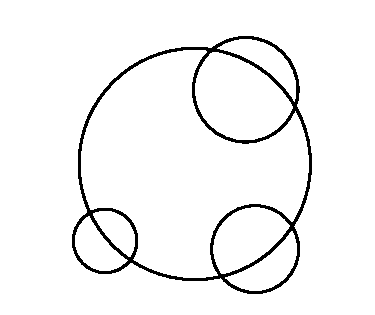
\includegraphics[scale = 0.4]{img/pivote_variante1}}\qquad\qquad
	\subfigure[El símbolo anarquista]{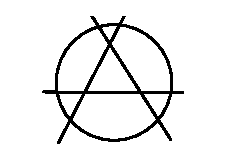
\includegraphics[scale = 0.8]{img/pivote_variante2}}
	\caption{Ilustración de conjuntos en las hipótesis de \ref{conex_cor_pivote_corte_comun}.}
\end{figure}

\begin{cor}[Cadenas]
	Sea una cadena finita $\{A_i\}_{i=1}^n$ de conexos, es decir, que verifica que $A_i\cap A_{i+1}\not=\emptyset$. Entonces $\bigcup_{i=1}^n A_i$ es conexo.
\end{cor}
\begin{proof}
	Por inducción, es claro que aplicando el teorema del pivote la cadena de dos eslabones $A_1\cup A_2$ es conexa, si suponemos que la cadena de $n$ eslabones es conexa, por el teorema del pivote, la de $n+1$ eslabones $A_{k+1}\cup\bigcup_{i=1}^k A_i$ lo será también.
\end{proof}
\begin{figure}[H]
	\centering
	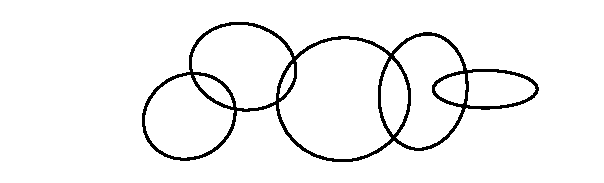
\includegraphics[scale = 0.5]{img/pivote_variante3}
	\caption{Ilustración de una cadena de conexos}
\end{figure}
\begin{obs}
	El corolario anterior también se verifica si la sucesión de conjuntos es numerable, pero no lo vamos a probar aquí.
	% AQUÍ VIENE PROBADO http://dbfin.com/topology/munkres/chapter-3/section-23-connected-spaces/problem-2-solution/
\end{obs}

El siguiente resultado, aunque también es consecuencia del teorema del pivote \ref{conex_theo_pivote}, es más que un mero corolario y merece la categoría de teorema por sí mismo.

\begin{theo}[Sandwich]\label{conex_teo_adherencia_conexa}
	Sea $A$ conexo y $B$ un conjunto emparedado entre $A$ y su adherencia, es decir, $A\subset B\subset\adher{A}$. Entonces $B$ es conexo. En particular, $\adher{A}$ es conexo.
\end{theo}
\begin{proof}
	Podemos poner nuestro conjunto $B$ de forma amigable para usar el teorema del pivote.
	\[B=\bigcup_{b\in B\setminus A} (A\cup\{b\}) \]
	como la intersección de la familia es no vacía, entonces basta probar que cada $A\cup\{b\}\subset\adher{A}$ es conexo, pues en ese caso el teorema del pivote \ref{conex_theo_pivote} nos garantiza la conexión de $B$.
	
	Si hubiera un clopen no trivial $C\subset A\cup\{b\}$, entonces, $C\cap A$ sería un clopen en $A$. Como $A$ es conexo, $C\cap A$ debe ser el vacío o el total.
	\begin{itemize}
		\item Si es el vacío, entonces $C=\{b\}$ y por tanto $\{b\}$ es abierto, luego, como el entorno $\{b\}$ de sí mismo no corta con $A$, $b\not\in\adher{A}$, lo cual es una contradicción.
		\item Si es el total, $C=A$ y por tanto $A$ es cerrado, pero $b\not\in A=\adher{A}$, que de nuevo es una contradicción. \qedhere
	\end{itemize}
\end{proof}

Recojamos los frutos de nuestra cosecha con un ejemplo, pero antes presentemos unas definiciones que harán más ágil nuestro discurrir.
\begin{defi}[Segmento]
	En $\R^n$ un segmento que une dos puntos $a$ y $b$ es el conjunto $\{ta+(1-t)b\midc t\in[0,1]\}$, que puede interpretarse como la imagen de la interpolación lineal entre $a$ y $b$, que definimos en la ecuación \eqref{interpolacion}.
\end{defi}
\begin{defi}[Convexo]
	En $\R^n$, se dice que un conjunto es \tbi{convexo} si para cada par de puntos $a,b\in E$, el segmento que los une también está en el conjunto.
\end{defi}
\begin{defi}[Estrellado]
	En $\R^n$ definimos conjunto \tbi{estrellado} como un conjunto en el que existe un punto tal que el segmento de él a cualquier otro está en el conjunto.
\end{defi}

\begin{exa}[Miscelánea]
	\label{conex_exa_miscel}
	Veamos algunos ejemplos de conjuntos conexos:
	\begin{enumerate}
		\item Los segmentos son conexos por ser la imagén continua de $[0,1]$, que es conexo, por la interpolación lineal, que es continua.
		\item Si un conjunto es convexo entonces es estrellado, y si es estrellado entonces es conexo. Además, las implicaciones recíprocas no se verifican. En resumen
		\[\text{Convexo}\ra\text{Estrellado}\ra \text{Conexo}\]
		
		En efecto, si $A$ es convexo tomando cualquier punto como ``centro de la estrella'' se deduce que $A$ es estrellado.
		
		Asimismo, si $A$ es estrellado se puede escribir como
		\[A=\bigcup_{a\in A} [a_0, a]\]
		para cierto $a_0\in A$. Cada segmento $[a_0,a]$ es conexo, y, por tanto, por el teorema del pivote, como todos comparten el punto $a_0$, su unión es conexa.
		
		Nótese que ni la convexidad ni ser estrellado son propiedades topológicas; ambas son propiedades vectoriales: su definición solo tiene sentido en un espacio que, al menos, tenga estructura de espacio vectorial.
		
		\item Una circunferencia en $\R^2$ es conexa, pero no es estrellada. En efecto, es conexa por ser la imagen de $[0,2\pi]$ por la aplicación $t\mapsto (\cos t, \sen t)$.
		
		\item El grafo de la función $\sen\frac{1}{x}$ para $x>0$, que escribimos:
		\[C = \left\{\left(x,\sen\frac{1}{x}\right)\midc x>0\right\}\]
		es conexo por ser la imagen continua de $(0,\infty)$ por la aplicación:
		\[x\mapsto \left(x,\sen\frac{1}{x}\right)\]
		
		Lo que es más interesante, para cualquier $a\in [-1,1]$ se verifica que $\{(0,a)\}$ es adherente a $C$ (es relativamente fácil de comprobar) y por tanto que $C\cup\{(0,a)\}$ es conexo.
		\begin{figure}[H]
			\centering
			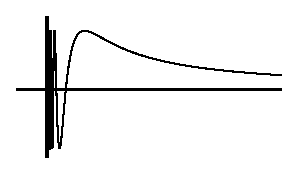
\includegraphics[scale = 0.8]{img/funcionsen1x}
			\caption{Ilustración de la gráfica de $\sen(1/x)$}
		\end{figure}
		
		\item Consideramos el conjunto:
		\begin{equation}\label{lineas}C = \big(\{0\}\times (0,1]\big) \cup \left(\bigcup_{n\in\N} [0,1]\times\left\{\frac{1}{n}\right\}\right) \end{equation}
		\begin{figure}[H]
			\centering
			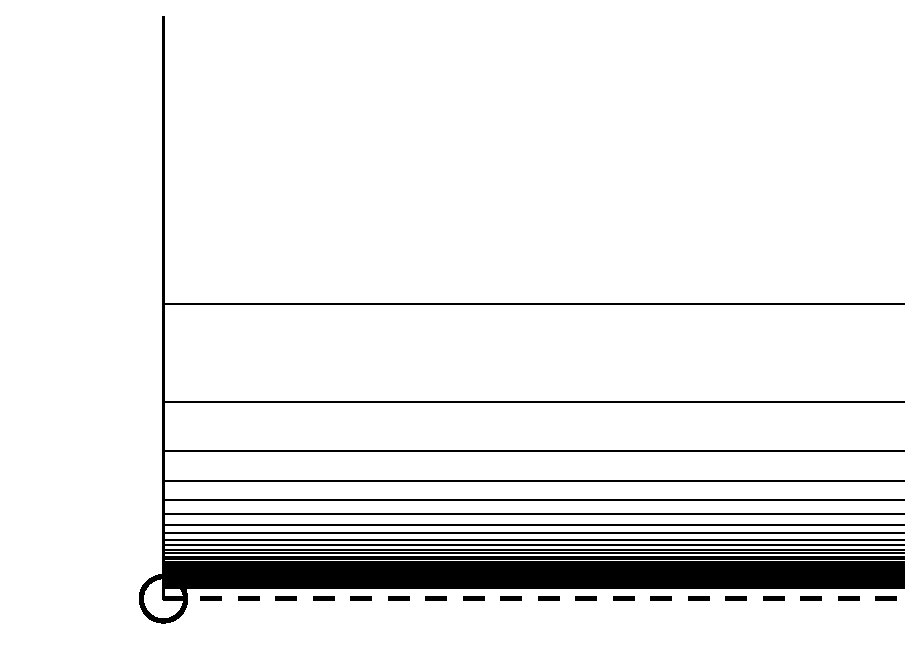
\includegraphics[scale = 0.2]{img/lineas}
			\caption{Ilustración del conjunto de la ecuación \eqref{lineas}}
		\end{figure}
		que es unión de segmentos horizontales cada vez más juntos y de un segmento vertical. Este es trivialmente conexo por el corolario \ref{conex_cor_pivote_corte_comun}. Lo particular es que si unimos a $C$ el segmento horizontal:
		\[(0,1)\times\{0\}\]
		sigue siendo conexo por ser adherencia de $C$ (¡compruébese!). 
\qedhere
	\end{enumerate}
\end{exa}

Completamos esta sección con una propiedad interesante garantizada por la conexión.

\begin{lem}[Cadena]
	Sea $\X$ conexo y $\{U_i\}_{i\in I}$ un recubrimiento por abiertos de $\X$. Dos puntos cualesquiera $x,y\in\X$ se pueden conectar mediante una cadena finita de abiertos del recubrimiento.
\end{lem}

\begin{proof}
	Sea $A=\{z\in\X \midc \text{existe una cadena de } x \text{ a } z \}$. $A$ es claramente no vacío, puesto que $x\in A$. Por ende, nuestro objetivo será ver que $\X=A$. Una forma de hacerlo será ver que $A$ es un clopen, ya que si lo fuera, por conexión de $\X$ y por ser $A$ no vacío $A$ tendría que ser el total.
	\begin{itemize}
		\item Veamos que $A$ es abierto. En efecto, dado $z\in A$, queremos ver que existe un abierto $U$ tal que $z\in U\subset A$. Si tomamos el último abierto $U$ de la cadena que une $x$ y $z$ hemos ganado, ya que $U\subset A$, ya que todo punto de $U$ queda unido con $x$ con la misma cadena que $z$.
		
		\item Ahora la clausura. En efecto, si $z\in\adher{A}$, entonces habrá un abierto $U_{i_0}$ tal que $U_{i_0}\cap A\not=\emptyset$. Considerando un punto $y$ de la intersección, como $y$ está en $A$, hay una cadena de $x$ a $y$. Uniendo $U_{i_0}$ a la cadena obtenemos una cadena de $x$ a $z$, y por tanto $z\in A$, luego $A=\adher{A}$. \qedhere
	\end{itemize}
\end{proof}
Este último resultado tiene una aplicación muy importante en los espacios euclídeos usuales.
\begin{defi}[Poligonal]
	Una \tbi{poligonal} en $\R^n$ es un conjunto $\Gamma$ de la forma\begin{equation*}
		\Gamma=[x_0,x_1]\cup[x_1,x_2]\cup\dots\cup[x_{n-2},x_{n-1}]\cup[x_{n-1},x_n]
	\end{equation*}
	Donde $[x_i,x_j]$ representa el segmento que une a los puntos $x_i$ y $x_j$. Nótese que por la variante de las cadenas del teorema del pivote una poligonal es conexa.
\end{defi}
\begin{defi}[Conexión por poligonales]
	Un conjunto $A\subset\R^n$ se dice \tbi[conexo!por poligonales]{conexo por poligonales} si dados dos puntos cualesquiera $x,y\in A$, hay una poligonal $\Gamma$ contenida en $A$ que une a $x$ y a $y$.
\end{defi}
\begin{obs}[Conexión y conexión por poligonales]
	Todo conjunto conexo por poligonales es conexo. En efecto, si tomamos un punto $a$ de $A$ y consideramos la familia de poligonales (conexos) que conectan a $a$ con el resto de puntos de $A$, tenemos que dicha familia tiene a $\{a\}$ por intersección, luego podemos aplicar el teorema del pivote, obteniendo que la unión de la familia, que es $A$, es conexa.
\end{obs}
\begin{obs}[Abiertos y conexión por poligonales]
	Podemos recubrir cualquier abierto conexo de $\R^n$ con bolas (véase el lema \ref{etop_lem_otrasProp}), y, por tanto existe una cadena de bolas que une cualquier par de puntos.
	
	Si tomamos un punto en cada intersección entre bolas consecutivas de la cadena y consideramos los segmentos que los unen, tengo una poligonal que conecta los dos puntos.
	
	De esta forma, para abiertos de $\R^n$ la conexión y la conexión por poligonales son nociones equivalentes.
\end{obs}

\section{Componentes conexas}

Al igual que ocurría con la compacidad, sería deseable que todos los espacios fuesen conexos. Dado que esto no se da, nos conformaremos con quedarnos con los subconjuntos conexos del espacio. Surge así la idea de componente conexa que definimos a continuación.

Aunque parezca que esto no es una ventaja, es tremendamente útil a la hora de estudiar, por ejemplo, si dos espacios son homeomorfos, ya que el número de componentes conexas se conserva por homeomorfismos (ver ejemplo \ref{etop_exa_homeomorfismos}).

\begin{defi}[Componente conexa de un punto]
	Se dice que un conjunto $\Co(x)\subset\X$ es una \tbi{componente conexa} de $x\in\Co(x)$ si es un conjunto conexo ``maximal''. Esto es que, dado un conjunto $D$ conexo que contiene a $x$ se verifica que $\Co(x)\not\subset D$.
	
	En general, diremos que un conjunto $\Co$ es una componente conexa si lo es de alguno de sus puntos (y por tanto de todos, véase la observación \ref{conex_obs_compartido}).
\end{defi}

Análogamente a lo que hicimos con el interior y la adherencia en el capítulo \ref{etop}, veamos que la componente conexa de un punto tiene una caracterización conjuntista muy sencilla.

\begin{lem}[Caracterización conjuntista]
	Dado $x\in\X$, el conjunto 
	$\Co(x)=\bigcup_{A\subset\X} A$ con $x\in A$ y $A$ conexo, es una componente conexa de $x$.
\end{lem}
\begin{proof}
	En efecto, $\Co(x)$ es no vacío, ya que $\{x\}$ es conexo. Además, la familia de conexos que conforma $\Co(x)$ tiene al menos a $\{x\}$ en la intersección, luego, por el teorema de pivote, $\Co(x)$ es conexo.
	
	Por construcción es, además, maximal, ya que, si hubiera un conexo que lo contuviera, este contendría a $x$, y, por tanto, estaría $\Co(x)$.
\end{proof}
\begin{obs}[Unicidad]
	\label{conex_obs_unicidad}
	Cabe destacar que $\Co(x)$ no es solo una componente conexa de $x$, sino \tb{la} componente conexa de $x$. 
	
	En efecto, si hubiera otra, digamos $E$, tanto $\Co(x)$ como $E$ deben contener a $x$, luego su intersección será no vacía $E\cap \Co(x)\not=\emptyset$. En tal caso, $A:=E\cup \Co(x)$ sería conexo por el teorema del pivote, y, como además $x\in A$, $A$ estará en la familia que conforma $\Co(x)$, luego $E\subset\Co(x)$. Como $E$ es una componente conexa se debe dar la igualdad.
\end{obs}
\begin{obs}[Intersección y contención]
	\label{conex_obs_inter}
	La observación \ref{conex_obs_unicidad}, a parte de darnos la unicidad de la componente conexa de un punto, nos viene a decir, que si un conexo corta a la componente conexa, este debe estar contenido en ella. Este hecho puede sacarnos de algún que otro apuro. 
\end{obs}
\begin{obs}[Componente conexa compartida]
	\label{conex_obs_compartido}
	Nótese que pudiera haber varios puntos con la misma componente conexa, de hecho, todos los puntos de $\Co(x)$ tienen a $\Co(x)$ por componente conexa. En efecto, sea $y\in\Co(x)$, llamemos $\Co(y)$ a su componente conexa. Es claro que, por la caracterización conjuntista $\Co(x)\subset\Co(y)$, luego, $x\in\Co(y)$, $\Co(y)$ es un conexo que contiene a $x$, por tanto, debe estar contenido en su componente conexa, es decir $\Co(y)\subset\Co(x)$.
	
	En definitiva podemos concluir que una componente conexa lo es de todos sus puntos y de ninguno más (obviamente). En particular, si un espacio es conexo, es la componente conexa de todos sus puntos.
\end{obs}

A continuación enunciamos y demostramos algunas propiedades de las componentes conexas.

\begin{lem}[Propiedades varias]
	Sea $\X$ un espacio topológico, entonces:
	\begin{enumerate}
		\item Las componentes conexas son cerradas.
		
		\item Las componentes conexas son una partición del espacio. Es decir, son disjuntas dos a dos y su unión es el total.
		
		\item Si $\X$ tiene un número finito de componentes conexas, estas son abiertas.
		\item Si en $\X$ todo punto tiene un entorno conexo, entonces las componentes conexas de $\X$ son abiertas.
	\end{enumerate}
\end{lem}
\begin{proof}
	Demostremos esto como si fuéramos a emparedar a alguien, ladrillo a ladrillo, en este caso, apartado a apartado.
	\begin{enumerate}
		\item Sea $\Co(x)$ componente conexa. Como es conexo, su adherencia es conexa ( véase el teorema del sandwich \ref{conex_teo_adherencia_conexa}), y por ser maximal $\Co(x)=\adher{\Co(x)}$.
		
		\item Es claro que
		\[\X=\bigcup_{x\in\X} \Co(x)\]
		Además, dadas dos componentes conexas, $\Co_1$ y $\Co_2$, si $\Co_1\cap\Co_2\not=\emptyset$ entonces $\Co_1\subseteq\Co_2$ y por ser maximales se daría la igualdad.
		
		\item Por hipótesis $\X=\Co_1\cup\cdots\cup\Co_r$ siendo la unión disjunta. Entonces, para cada $i\in\{1,\cdots r\}$ se tiene que 
		\[\Co_i=\X\setminus (\Co_1\cup\cdots\cup\Co_{i-1}\cup\Co_{i+1}\cup\cdots\cup\Co_r)=:\X\setminus \Co\]
		Como cada componente conexa es cerrada, y además, la unión finita de cerrados es cerrada, $\Co$ es cerrado, luego como $\Co_i=\X\backslash \Co$, es claro que $\Co_i$ es abierto para todo $i$.
		
		\item Sea $\Co$ componente conexa de $\X$, veamos que es entorno de todos sus puntos. Sea $x\in\Co$. Por hipótesis existe $\V$ entorno conexo de $x$, con lo cual $\V\cap\Co\not=\emptyset$. Esto implica que $x\in\V\subset\Co$, con lo que $\Co$ es entorno de $x$.\qedhere
	\end{enumerate}
\end{proof}
Veamos ahora una serie de ejemplos para familiarizarnos con estos conceptos.
\begin{exa}[Sucesión armónica]
	Estudiemos las componentes conexas del espacio topológico compuesto por el rango de la sucesión armónica y su límite $\X:=\{0\}\cup\{1/n\midc n\in\N\}$.
	
	Evidentemente, los puntos son conexos, el reto será pues, ver si puede haber una componente conexa $\Co$ con dos puntos distintos, digamos $x$ e $y$, sin pérdida de generalidad $x<y$.
	
	Si $\Co$ fuera conexo, por la caracterización de los conexos de la recta, debería contener a todos sus puntos intermedios, no obstante es claro que $y=1/n_0$ para cierto $n_0\in\N$, luego tomando el punto medio $c$ entre $\frac{1}{n_0+1}$ e $y$ tenemos que $c$ es un punto entre $x$ e $y$ que no está en $\X$ y por tanto no está en $\Co$. Luego los únicos conexos de $\X$ son los puntos.
	
	Además, se comprueba fácilmente que las componentes conexas de $\{1/n\midc n\in\N\}$ son abiertas, no obstante la componente conexa $\{0\}$ no es abierta (¡compruébese!).
\end{exa}
Razonando de manera similar podemos estudiar las componentes conexas de $\Q$.
\begin{exa}[Racionales] Por densidad de $\Q$ en $\R$ entre dos irracionales siempre hay un racional, luego las únicas componentes conexas de $\Q$ son los puntos. Además, ninguna de estas componentes es abierta. Esto último también se deduce de la densidad de $\Q$.
\end{exa}
Los dos ejemplos anteriores estudiaban las componentes conexas de espacios numerables, viendo que las únicas componentes conexas eran los propios puntos. Nos preguntaremos si pudiera ocurrir esto también con espacios no numerables.
\begin{exa}[Discontinuo de Cantor]
	Aunque no lo demostraremos aquí, el conjunto de Cantor $K$, que tantas propiedades nos esconde, es no numerable y sus componentes conexas son los puntos. 
\end{exa}
Veamos otro ejemplo (esta vez más sencillo) de este fenómeno.
\begin{exa}[Sorgenfrey]
	La recta de Sorgenfrey tiene por componentes conexas a los puntos, esto se debe, como veremos en el lema \ref{conex_baseClop}, a que la recta de Sorgenfrey es \kolmogorov (de hecho \hausdorff) y tiene una base de clopens (ver ejemplo \ref{etop_sorgenfrey}).  
\end{exa}
A la luz de este último ejemplo, brota cual tubérculo el siguiente lema.
\begin{lem}[Bases de clopens]
	\label{conex_baseClop}
	Si $\X$ es \kolmogorov y tiene una base $\B$ de clopens, entonces sus componentes conexas son los puntos, es decir, es \tbi{totalmente disconexo}.
\end{lem}
\begin{proof}
	Si hubiera un conexo $A$ con dos puntos distintos, digamos $a$ y $b$, al ser $\X$ \kolmogorov, habrá un entorno $B$ en $A$, sin pérdida de generalidad de $a$, que podremos tomar básico (luego clopen), tal que no contiene a $b$. Luego $b\in A\setminus B$. Como $B$ es clopen, $A\setminus B$ también lo será. Luego acabamos de particionar $A$ con dos clopens no triviales, en contra de su conexión.
\end{proof}
\section{Comportamiento de la conexión}
Llegados a este punto, para estudiar el comportamiento topológico no tenemos que hacer prácticamente nada. En efecto, veámoslo punto por punto.
\begin{itemize}
	\item Es claro que la conexión no se traslada a subespacios (no todos los subconjuntos de $\R$ son intervalos).
	\item Por su parte, como la imagen continua de conexos es conexa, los cocientes, que no son más que imágenes continuas drásticas, serán también conexos.
	\item En cuanto a la suma, ya demostramos en la observación \ref{const_obs_propiedadesSuma} que cada sumando era un clopen, luego ya en el caso de espacios suma de dos sumandos obtenemos una partición del conjunto en dos clopens. Luego la suma nunca es conexa.
\end{itemize}
Demostremos ahora con más calma que el producto de espacios conexos es conexo, para lo cual usaremos a nuestro querido teorema del pivote.
\begin{prop}[Conexión y productos]
	Si $\X$ e $\Y$ son conexos, entonces $\X\times \Y$ es conexo.
\end{prop}
\begin{proof}
	Para cualquier $x\in \X$ e $y\in \Y$ es claro que $A_y:=\X\times\{y\}$ y $B_x:=\{x\}\times \Y$ son conjuntos conexos por ser copias homeomorfas de $\X$ e $\Y$ respectivamente. Además, se tiene $A_y\cap B_x=(x,y)$, luego no vacía. Aplicando el teorema del pivote tenemos que $C_{(x,y)}=A_y\cup B_x$ es conexo. Tomando la familia de estos conjuntos, que es claro que se intersecan dos a dos y cubren el espacio, podemos aplicar el corolario \ref{conex_cor_pivote_corte_comun} para deducir que $\X\times \Y$ es conexo.
\end{proof}
Recapitulemos todo lo visto con una tabla.
\begin{table}[H]
	\centering
	\begin{tabular}{l|l|l|l|l|}
		\cline{2-5}
		& \textbf{Subespacios}    & \textbf{Cociente}       & \textbf{Producto}       & \textbf{Suma}           \\ \hline
		\multicolumn{1}{|c|}{\textbf{Conexión}} & \multicolumn{1}{c|}{No} & \multicolumn{1}{c|}{Sí*} & \multicolumn{1}{c|}{Sí} & \multicolumn{1}{c|}{No} \\ \hline
	\end{tabular}
	\caption{Tabla resumen de conexión.}
	\label{Tabla_conexion}
\end{table}
\section{Local--conexión}
Vamos a definir la conexión local basándonos en la filosofía de la compacidad local.
\begin{defi}[Conexión local]
	Un espacio $\X$ se dice localmente conexo si cada uno de sus puntos tiene una base de entornos conexos.
\end{defi}
Presentemos un criterio general que caracteriza a los espacios localmente conexos.
\begin{prop}[Caracterización] Las siguientes afirmaciones son equivalentes
	\begin{enumerate}
		\item $\X$ es localmente conexo.
		\item Las componentes conexas de todo abierto de $\X$ son abiertas.
		\item Todo punto de $\X$ tiene una base de entornos conexos y abiertos.
	\end{enumerate}
\end{prop}
\begin{proof}Realicemos el habitual círculo económico de implicaciones.
	\begin{enumerate}[align=left, leftmargin=*]
		\item[\fbox{$(1)\ra (2)$}] Sea $G$ un abierto de $\X$ y $\Co$ una componente conexa de $G$. Sea $x\in \Co$, al ser $G$ abierto, es entorno de todos sus puntos, y, por ser $\X$ localmente conexo, habrá un $\V$ entorno conexo de $x$ tal que $x\in \V\subset G$. Como $V\cap\Co\not=\emptyset$ ya que $x$ está en ambos conjuntos, y al ser $\Co$ la componente conexa de $x$ se tiene que $V\subset\Co$, con lo que se tiene el resultado.
		\item[\fbox{$(2)\ra (3)$}] Dado $x\in\X$, consideremos el conjunto de sus entornos abiertos conexos $\Va{x}$, veamos que es una base de entornos. En efecto, dado un entorno abierto de $x$, digamos $U$, $x$ estará en alguna de las componentes conexas $\Co$ de $U$, que por hipótesis son abiertas, luego $\Co\in\Va{x}$.  
		\item[\fbox{$(3)\ra (1)$}] Es evidente.\qedhere
	\end{enumerate}
\end{proof}
\section{Comportamiento de la local--conexión}
Lamentablemente, el estudio del comportamiento topológico de la conexión local no será tan sencillo como el de la conexión. Sin embargo a estas alturas ya no debería importarnos mucho, el lector ya debería estar curado de espanto.

En primer lugar cabe destacar que la imagen continua de un conjunto localmente conexo no necesariamente es localmente conexo. Sin embargo, la local--conexión se hereda a los cocientes.
\begin{prop}[Local--conexión y cocientes]
	Sea $\X$ localmente conexo y $f:\X\to\Y$ una identificación. Entonces, $\Y$ es localmente conexo.
\end{prop}
\begin{proof}
	Para comprobar esto echaremos mano de la caracterización de la local--conexión y comprobaremos que las componentes conexas de los abiertos de $\Y$ son abiertas.
	
	Sea $G$ un abierto de $\Y$ y $\Co$ una componente conexa de $G$. Como $f$ es una identificación $\Co$ será abierta si y solo si $f^{-1}(\Co)$ es abierto. Sea pues $x\in f^{-1}(\Co)$.
	
	Al ser $f$ continua $f^{-1}(G)$ es abierto. Como $\X$ es localmente conexo, habrá un entorno conexo $V$ que verifique que $x\in V\subset f^{-1}(G)$. Si aplicamos $f$ a la última desigualdad, al ser $f$ sobreyectiva se tiene que $f(V)\subset G$, siendo $f(V)$ un conexo contenido en $G$ por ser $f$ continua.
	
	Como tanto $f(V)$ como $\Co$ contienen a $f(x)$ es claro que se cortan, luego por la observación \ref{conex_obs_inter} se verifica que $f(x)\in f(V)\subset \Co$, con lo que $\Co$ es entorno de todos sus puntos.
\end{proof}
Aunque la conexión local se comporta peor que la conexión con los cocientes, se comporta un poco mejor con los subespacios, no llegándose a heredar la local--conexión a todos ellos.
\begin{lem}[Subespacios y local--conexión]
	Si $A$ es un subespacio abierto de $\X$, siendo $\X$ localmente conexo, entonces $A$ es localmente conexo.
\end{lem}
\begin{proof}
	Como $x$ tiene una base de entornos $\Va{x}$ conexos abiertos, tomando la base relativa $\Va{x}\cap A$, veamos que es de entornos conexos.
	
	Como $U$ es abierto en $A$ si y solo si lo es en $\X$ (véase el lema \ref{etop_lem_otrasProp}), si no hay dos abiertos en $\X$ que particionen a los entornos de $\Va{x}$, tampoco los habrá que partan a los entornos $\Va{x}\cap A$, ya que es la subfamilia de los entornos de $\Va{x}$ contenidos en $A$.
\end{proof}
\begin{obs}[Contraejemplo]
	Para ver que la conexión local no se hereda en general, basta ver que $\R$ es localmente conexo ya que cada punto posee una base de intervalos, pero su subespacio $\{1/n\midc n\in\N\}\cup\{0\}$ no es localmente conexo al no tener $0$ una base de entornos conexos y abiertos. Esto es claro ya que el único conexo que es entorno de $0$ es el propio $\{0\}$, que no es abierto (¡compruébese!).
\end{obs}
Ahora le toca el turno a los productos y las sumas, que estudiaremos brevemente.
\begin{itemize}
	\item El producto de espacios localmente conexos es localmente conexo, esto se debe a que las bases de entorno del producto son productos de bases de entornos de los factores. Tomando la base de conexos correspondiente de cada factor, como el producto de conexos es conexo, se tiene el resultado.
	\item La suma de espacios localmente conexos es localmente conexa.
	
	En efecto, tomando un punto cualquiera $x$ del espacio suma, este estará en alguno de los estantes, que son homeomorfos a los sumandos vía las inclusiones. Como los sumandos son localmente conexos, $p_i^{-1}(x)$ tiene una base de entornos conexos, que se transforma por $p_i$ en una base de entornos conexos de $x$ por ser $p_i$ continua. 
\end{itemize}
Condensando todo lo visto, presentamos el resumen en forma de tabla.
\begin{table}[H]
	\centering
	\begin{tabular}{l|l|l|l|l|}
		\cline{2-5}
		& \textbf{Subespacios}                                                                      & \textbf{Cociente}       & \textbf{Producto}       & \textbf{Suma}           \\ \hline
		\multicolumn{1}{|c|}{\textbf{\begin{tabular}[c]{@{}c@{}}Local\\ conexión\end{tabular}}} & \multicolumn{1}{c|}{\begin{tabular}[c]{@{}c@{}}Sí, en el caso\\ de abiertos\end{tabular}} & \multicolumn{1}{c|}{Sí} & \multicolumn{1}{c|}{Sí} & \multicolumn{1}{c|}{Sí} \\ \hline
	\end{tabular}
	\caption{Tabla resumen de local conexión}
	\label{Tabla_localconexion}
\end{table}
Presentamos para terminar un ejemplo con objeto de aumentar la curiosidad del lector.
\begin{exa}[Conexión local y por poligonales]
	El espacio $\X:=C\cup\{(0,0)\}$ donde $C$ es el conjunto definido en la ecuación \eqref{lineas} no es localmente conexo pero si es conexo por poligonales.
	
	La conexión por poligonales es evidente, dados dos puntos de $X$, si están en la misma recta horizontal basta con coger el segmento que los une.
	
	En caso contrario, bastaría con tomar el segmento horizontal que une al primer punto con $\{0\}\times [0,1]$, enlazándolo con el segmento vertical que llega hasta la altura del segundo punto, y, finalmente, enganchar este último al segmento horizontal que une $\{0\}\times [0,1]$ con el segundo punto. 
	
	La demostración de que no es localmente conexo es una adaptación de la demostración de que $\{1/n\midc n\in\N\}\cup\{0\}$ no es localmente conexo. Los detalles se dejan al lector.
\end{exa}
	
	\part{Topología algebraica}
	%Para este capítulo se usará la abreviatura "grf".
\chapter{Grupo fundamental}
\label{grf}

La topología algebraica comprende métodos que son significativamente distintos a los empleados hasta ahora en topología general. Intenta asignar a un espacio topológico algún invariante algebraico (por ejemplo, un grupo) y utilizar las propiedades de este invariante para obtener información sobre la topología. Este capítulo se centrará, pues, en el estudio del grupo fundamental, que es uno de estos invariantes.

\section{Homotopía}

En particular, introducimos la homotopía con el propósito de definir más adelante la noción de grupo fundamental. Dos caminos son, intuitivamente, homótopos si podemos deformar uno en el otro de forma continua.

% FALTA LA MAYORÍA DE LA SECCIÓN, EXCEPTO ESTE ÚLTIMO EJEMPLO	

\begin{exa}
	La interpolación lineal produce homotopías relativas. En efecto, consideramos la homotopía:
	\[H_s = (1-s)f + sg\]
	Si $f(a)=g(a)$ para algún $a\in\Y$, entonces resulta que:
	\[H_s(a)=(1-s)f(a)+sg(a)=f(a)=g(a)\]
	
	En particular, en $\R^n$, cualquier par de caminos cuyos extremos coincidan son homótopos con extremos fijos. De esta forma, en cualquier espacio $\X$ homeomorfo a $\R^n$ por un homeomorfismo $h:\R^n\to \X$, cualesquiera dos caminos cuyos extremos coincidan son homótopos con extremos fijos. En efecto, podemos fabricar la homotopía fácilmente: sean $\sigma,\tau$ los caminos en $\X$. Consideramos $\alpha,\beta$ caminos en $\R^n$, de forma que verifiquen que $\sigma = h\circ\alpha$, $\tau = h\circ\beta$. Como $\alpha$ y $\beta$ comparten extremos y están en $\R^n$, son homótopos con extremos fijos, y dada la homotopía $H_s$, resulta que $h\circ H_s$ es homotopía entre $\sigma$ y $\tau$.
\end{exa}

\section{Esferas}

El estudio de las homotopías en las esferas es interesante como ejemplo, y permite, basándose tan solo en lo visto en la anterior sección, demostrar un resultado no trivial.

Empezamos definiendo formalmente la esfera, para aclarar la notación.

\begin{defi}[Esfera]
	Llamamos \tbi{esfera} de dimensión $n$ y denotamos $\Sfe^n$ al subconjunto de $\R^{n+1}$:
	\[\Sfe^n = \{x\in\R^{n+1}\midc \norm{x}=1\}\subset\R^{n+1}\]
	donde $\norm{\cdot}$ es la norma euclídea. Cuando se considera como espacio topológico es con la restricción de la topología usual, si no se especifica otra.
\end{defi}

\begin{obs}
	Si bien la esfera de la definición anterior es la esfera unidad, nótese que todas las esferas de cualquier radio y centradas en cualquier punto de $\R^{n+1}$ son homeomorfas a la esfera que hemos definido.
\end{obs}

El resultado no trivial que mencionábamos en la introducción de esta sección es el siguiente:

\begin{prop}
	\label{grf_homotop_caminos_esfera}
	Dos caminos en una esfera $\Sfe^n$, $n\geq 2$, que tengan los mismos extremos son homótopos con extremos fijos.

	\begin{proof}
		% TODO: demostración
		Falta
	\end{proof}
\end{prop}

Un resultado muy relacionado ha sido un problema abierto hasta hace muy poco tiempo:

\begin{conjet}[Poincaré]
	La propiedad de la proposición \ref{grf_homotop_caminos_esfera} caracteriza a la esfera $\Sfe^3$. Esto es, si un espacio topológico verifica que cualquier par de caminos en él que tengan los mismos extremos son homótopos con extremos fijos, entonces es homeomorfo a la esfera unidad.
\end{conjet}

La versión generalizada de esta conjetura, para la esfera $\Sfe^n$, también es cierta y tiene interés. Históricamente:
\begin{itemize}
	\item Para $n=2$, el resultado se conoce desde el siglo XIX.
	\item Para $n=5$, Zeeman lo demostró en 1961.
	\item Para $n\geq 6$, Smale lo demostró en 1961.
	\item Para $n=4$, Donaldson lo demostró en 1985.
	\item Para $n=3$, la versión original de la conjetura, Perelman lo demostró en 2006. La conjetura era uno de los 7 problemas del milenio, dotados con 1.000.000\$. Perelman rechazó tanto este premio como la medalla Fields tras demostrar la conjetura.
\end{itemize}
	
	\appendix
	\part{Apéndices}
	%Provisional
\chapter{Espacios Métricos}
\label{met}
En este apéndice veremos con detalle las relaciones entre los archiestudiados espacios métricos con los espacios topológicos.
% Mazo Por Hacer (Algún Día)
\section{Normas}
En esta comentamos (entre otras cosas) algunos resultados interesantes (y bonitos) sobre normas que usualmente se usan como mantras satánicos (pues jamás se demuestran).
\subsection{Conceptos Previos}
A continuación introducimos la definición de norma y los conceptos que a ella subyacen.
\begin{defi}[Norma]
	Es harto conocido, casi desde que Eduardo Aguirre\footnote{En la mitología de los Dobles Grados, profesor de Álgebra Lineal conocido por sus refranes y frases célebres.} llevaba pantalones cortos, que una \tbi[norma]{norma} es una aplicación $\norm{\cdot}:E\to\K$ que verifica
	\begin{enumerate}
		\item \label{norma_vector_nulo} Es nula si y solo si el vector es nulo. Es decir, dado $u\in\R^n$
		\begin{equation*}
			\norm{u}=0\sii u=0
		\end{equation*}
		\item \label{norma_lambda} Tiene un comportamiento lineal respecto a escalares. Esto es
		\begin{equation*}
		\norm{\lambda u}=\abs{\lambda}\norm{u}
		\end{equation*}	
		\item \label{norma_triangular} Verifica la desigualdad triangular o de Minkowski, es decir, dados dos vectores $u,v\in\R^n$
		\begin{equation*}
		\norm{u+v}\le \norm{u}+\norm{v}
		\end{equation*}
	\end{enumerate}
\end{defi}
Una definición que surge de forma automática es la de espacio vectorial normado.
\begin{defi}[Espacio Vectorial Normado]
	Llamamos \tbi[espacio vectorial normado]{espacio vectorial normado} a un espacio vectorial $E$ equipado con una norma $\norm{\cdot}$, es decir, al par $(E,\norm{\cdot})$.
\end{defi}
\subsection{Topologización de un Espacio Vectorial Normado}
Todo espacio vectorial normado puede ser ``metrizado'' de forma canónica, tal y como muestra la siguiente definición.
\begin{defi}[Métrica Procedente de la Norma]
	Decimos que una métrica $d$ definida sobre un espacio vectorial $E$ \tbi[métrica!procedente de una norma]{procede de una norma} si existe una norma $\norm{\cdot}$ tal que cumple
	\begin{equation*}
		d(x,y)=\norm{x-y}
	\end{equation*}
\end{defi}
Así, como todo espacio métrico es, a su vez, un espacio topológico (ver ejemplo \ref{etop_exa_topologias}), podemos preguntarnos qué relaciones hay entre las topologías engendradas por dos normas. En particular, cabe preguntarse cuándo dos normas generan la misma topología.
\begin{defi}[Equivalencia de Normas]
	Decimos que dos normas $\norm{\cdot}_1$ y $\norm{\cdot}_2$ son \tbi[norma!equivalente]{equivalentes} si engendran la misma topología.
\end{defi}
\subsection{Teorema General de Equivalencia}
Esta sección está dedicada a demostrar el siguiente teorema.
\begin{theo}[Teorema General de Equivalencia]
	Sea $E$ un espacio vectorial del dimensión finita $n$. Entonces, todas las normas definidas sobre $E$ son equivalentes.
\end{theo}
Como la demostración del teorema es un poco larga (tampoco demasiado), la dotaremos de una sección propia.
\subsubsection{Demostración del Teorema General de Equivalencia}
Nuestro objetivo es, dadas dos normas arbitrarias, $\norm{\cdot}_1$ y $\norm{\cdot}_2$ de $E$, demostrar que las topologías engendradas por ellas son iguales. Es decir
\begin{equation*}
\T_{\norm{\cdot}_1}=\T_{\norm{\cdot}_2}
\end{equation*}
Para ello, estudiemos y repasemos algunas propiedades generales de las normas.

Otra propiedad a tener en cuenta es la continuidad. Dado que esta será crucial en la demostración, nos detendremos un poco más en ella.


Veamos que una norma $\norm{\cdot}$ es continua en la topología usual. Con esto último queremos decir que en $\R^n$ consideramos la topología definida por la distancia euclídea (que a su vez se define a partir de la norma euclídea $\norm{\cdot}_e$) y en $\R$ la topología definida por el valor absoluto.


Por tanto, para demostrar que una norma es continua en la topología usual debemos probar que, dado $a\in\R^n$ y dado $\varepsilon>0$, existe un $\delta>0$ tal que si 

\[x\in \bola_{\norm{\cdot}_e}(a,\delta)\]

entonces

\[f(x)=\norm{x}\in \bola_{\abs{\cdot}}(f(a),\varepsilon)=\bola_{\abs{\cdot}}(\norm{a},\varepsilon)\]

En otras palabras, dado $a\in\R^n$ y dado $\varepsilon>0$, existe un $\delta>0$ tal que si

\[\norm{x-a}_e<\delta\]

entonces

\[\abs{\norm{x}-\norm{a}}<\varepsilon\]


En efecto, aplicando las propiedades antes vistas, tenemos que

\begin{equation*}
\abs{\norm{x}-\norm{a}}\le \abs{\norm{x-a}}=\norm{x-a}=\norm{\sum_i(x_i-a_i)e_i}\stackrel{2.3.}{\le}\sum_i\abs{x_i-a_i}\norm{e_i}
\end{equation*}

Teniendo en cuenta que $\abs{x_i-a_i}\le \norm{x-a}_e$, queda

\begin{equation*}
\abs{\norm{x}-\norm{a}}\le \sum_i\norm{x-a}_e\norm{e_i}=\norm{x-a}_e\sum_i\norm{e_i}
\end{equation*}

donde $\sum_i\norm{e_i}$ es una constante que denotaremos por $C$.


Así, dado $\varepsilon>0$, existe $\delta=\varepsilon/C>0$ tal que si $\norm{x-a}_e<\delta$, entonces

\begin{equation*}
\abs{\norm{x}-\norm{a}}<\varepsilon
\end{equation*}

con lo que queda probada la continuidad de la norma $\norm{\cdot}$.\\



Ya tenemos todo lo necesario para realizar la demostración. Una vez que probemos las dos contenciones de las topologías, es decir

\begin{equation*}
\T_{\norm{\cdot}_1}\subset\T_{\norm{\cdot}_2} \ \ \text{y} \  \	\T_{\norm{\cdot}_1}\supset\T_{\norm{\cdot}_2}
\end{equation*}

habremos terminado. 


Comencemos notando que la función 

\begin{equation*}
\frac{\norm{\cdot}_1}{\norm{\cdot}_2}:\esfera^{n-1}\subset \R^n\rightarrow \R
\end{equation*}

es continua con la topología usual en $\esfera^{n-1}$, ya que el denominador no se anula y las normas son continuas. Dado que $\esfera^{n-1}$ es compacto, la función es acotada y alcanza el mínimo. Como el numerador tampoco se anula en el compacto, esto equivale a decir que existen $a,b>0$ tal que

\begin{equation*}
0<a\le \frac{\norm{\cdot}_1}{\norm{\cdot}_2}\le b
\end{equation*}

en $\esfera^{n-1}$. Es decir, para todo $v\in\esfera^{n-1}$ se tiene que

\begin{equation*}
0<a\norm{v}_2\le \norm{v}_1\le b\norm{v}_2
\end{equation*}

Lo deseable sería tener esta desigualdad para un vector cualquiera de $\R^n$ y así tener relacionadas las distancias de ambas topologías. Veamos que así es.


Sea $u\in\R^n\backslash\zset$, existe un vector $v\in \esfera^{n-1}$ y un número positivo $\lambda$ tal que $u=\lambda v$. Entonces, multiplicando por $\lambda$ en la desigualdad anterior, dado que es positivo, y utilizando la propiedad \ref{norma_lambda}, obtenemos

\begin{equation*}
a\lambda\norm{v}_2\le \lambda\norm{v}_1\le b\lambda\norm{v}_2\sii a\norm{\lambda v}_2\le \norm{\lambda v}_1\le b\norm{\lambda v}_2\sii a\norm{u}_2\le \norm{u}_1\le b\norm{u}_2
\end{equation*}

Por otro lado, si $u$ es el vector nulo, la desigualdad se cumple trivialmente. Por tanto, para todo vector $u$ de $\R^n$ se tiene que

\begin{equation}\label{desigualdad_normas}
a\norm{u}_2\le \norm{u}_1\le b\norm{u}_2
\end{equation}

donde $a,b>0$.\\



Por último, relacionemos los abiertos de ambas topologías para obtener las dos inclusiones. Una vez que tenemos la relación entre las normas, es fácil encontrar una relación entre las bolas de ambas topologías, dado que estas se definen a partir de las distancias que definen las normas.


Sea $x\in \bola_{d_1}(\rho,\varepsilon)$. Esto implica que $\norm{x-\rho}_1<\varepsilon$. Por la desigualdad \eqref{desigualdad_normas} se tiene entonces que $\norm{x-\rho}_2\le\varepsilon/a$, lo cual a su vez implica que $x\in \bola_{d_2}(\rho,\varepsilon/a)$. Es decir,

\begin{equation*}
\bola_{d_1}(\rho,\varepsilon)\subset \bola_{d_2}(\rho,\varepsilon/a)
\end{equation*}

Por tanto, dado $\U$ un abierto de la topología $\T_{\norm{\cdot}_2}$ siempre podemos encontrar un abierto de la topología $\T_{\norm{\cdot}_1}$ contenido en él. Esto es evidente ya que al ser $\U$ un abierto, contendrá una bola $\bola_{d_2}$ que a su vez, por lo que acabamos de ver, contiene una bola $\bola_{d_1}$, que es un abierto de $\T_{\norm{\cdot}_1}$. Esto implica que la topología definida por la norma $\norm{\cdot}_1$ tiene más abiertos, ya que al menos tiene uno por cada abierto de $\T_{\norm{\cdot}_2}$. Es decir, acabamos de demostrar que

\begin{equation*}
\T_{\norm{\cdot}_1}\supset\T_{\norm{\cdot}_2}
\end{equation*}


De la misma forma, dado $x\in \bola_{d_2}(\rho,\varepsilon)$, es decir, $\norm{x-\rho}_2<\varepsilon$, por la desigualdad \eqref{desigualdad_normas} se tiene que $\norm{x-\rho}_1<b\varepsilon$, lo cual implica que $x\in \bola_{d_1}(\rho,b\varepsilon)$. Es decir,

\begin{equation*}
\bola_{d_2}(\rho,\varepsilon)\subset \bola_{d_1}(\rho,b\varepsilon)
\end{equation*}


Razonando como acabamos de hacer, esto implica que

\begin{equation*}
\T_{\norm{\cdot}_1}\subset\T_{\norm{\cdot}_2}
\end{equation*}

Así, finalmente, se concluye que

\begin{equation}
\T_{\norm{\cdot}_1}=\T_{\norm{\cdot}_2}
\end{equation}

Dado que las normas eran arbitrarias, queda demostrado que todas las normas de $\R^n$ son equivalentes.

	\chapter{Funtores y teoría de categorías}
\label{funt}

Este anexo, si bien no es necesario para entender el apartado correspondiente, quiere ser una brevísima introducción (informal en algunos aspectos) a los conceptos más básicos de teoría de categorías, de forma que el lector comprenda qué es realmente un funtor y pueda aplicar este conocimiento a la topología algebraica, donde los utilizamos. 

Empezamos ``definiendo'' pues qué es una categoría, pero para ello hay que conocer antes el concepto de clase.

\section{Clases}

\begin{defi}[Clase]
Una \tbi{clase} es una colección de objetos (a menudo conjuntos, con una estructura adicional) que pueden ser definidos inequívocamente por una propiedad común. Por ejemplo, podemos considerar la clase de los grupos o la clase de los espacios vectoriales.
\end{defi}

\begin{obs}[Clase propia]
Decimos que una clase es \tb{\ti{propia}} si no es un conjunto. Desde luego, cualquier conjunto es una clase, lo cual se sigue directamente de la definición (la propiedad es que un elemento pertenece a la clase cuando pertenece al conjunto).

Así, de forma muy intuitiva, podemos considerar una clase propia como un ``conjunto muy grande''. Si se pudieran definir conjuntos como definimos clases propias, citando una propiedad común, introduciríamos paradojas en la teoría de conjuntos, como la archiconocida paradoja de Russell. De esta forma, se crea el concepto de clase, que trata de solventar este obstáculo. Por ejemplo, la paradoja de Russell no se da con clases porque no existe la noción de que una clase esté contenida en otra.

Nótese que en algunas teorías de conjuntos formales, y en particular con los axiomas ZFC, las clases no se definen. De esta forma, se aceptan en cuanto que todo lo que se formule con clases se pueda formular sin ellas, usando, en particular, la propiedad asociada, expresable con una fórmula. En este sentido, se pueden entender las clases como ``clases de equivalencia de fórmulas''.
\end{obs}

\section{Categorías y funtores}

Ahora sí, podemos definir una categoría. La definición puede variar según el autor, pero el concepto por detrás es siempre el mismo.

\begin{defi}[Categoría]
\label{funt_defi_categoria}

Una \tbi{categoría} consiste en:

\begin{itemize}
\item Una clase de \tb{\ti{objetos}} (a menudo conjuntos, con o sin estructura adicional).
\item Una clase de \tb{\ti{morfismos}}, que van de un objeto de los anteriores a otro. Un morfismo es una aplicación entre dos objetos que preserva su estructura. Por ejemplo, si los objetos son conjuntos los morfismos son funciones, si son grupos los morfismos son homomorfismos, y si los objetos son espacios topológicos los morfismos son funciones continuas.
\item Una operación de \tb{\ti{composición}}, que dados dos morfismos $f:a\to b$, $g:b\to c$ devuelva $g\circ f:a\to c$.
\end{itemize}

Y los siguientes axiomas:
\begin{enumerate}[label=\Roman*]
\item \tb{Asociatividad de la composición:} la composición de morfismos es asociativa. Es decir, $(f\circ g)\circ h=f\circ(g\circ h)$.
\item \tb{Morfismo identidad:} para cada objeto $x$, existe un morfismo $1_x:x\to x$ de forma que para cualquier $f:a\to x$ y $g:x\to b$, $1_x\circ f=f$ y $g\circ 1_x=g$.
\end{enumerate}
\end{defi}

\begin{obs}
	Es habitual referirse a las categorías con una abreviatura del nombre de la palabra en negrita. Así, la categoría de todos los grupos, donde los morfismos son los homomorfismos de grupos se denota \Grp. Se puede comprobar con facilidad que esta es, en efecto, una categoría.
\end{obs}

Ahora ya podemos definir el concepto de funtor.

\begin{defi}[Funtor]
\label{funt_defi_funtor}

Un \tbi{funtor} o \tb{\ti{functor}} es una aplicación $F:C\to D$ entre dos categorías $C$ y $D$ que asigna a cada objeto otro objeto y a cada morfismo otro morfismo de forma que preserva los morfismos identidad y la composición. Es decir, para cada $X\in C$, $F(\Id_X)=\Id_{F(X)}$; y para cada $f:X\to Y$ y $g:Y\to Z$, $F(g\circ f)=F(g)\circ F(f)$.
\end{defi}

\begin{obs}
Intuitivamente, un funtor es un homomorfismo para categorías: una aplicación que conserva la estructura de las categorías. En particular, la colección de categorías cuyos objetos son conjuntos (no son clases propias) es una categoría, y en este caso un funtor es él mismo un morfismo de esta categoría de categorías pequeñas.
\end{obs}

\section{\ti{General nonsense}}

La teoría de categorías tiene utilidad para abstraer otros conceptos matemáticos en muchas áreas. Su propósito es usar esta abstracción para poder probar resultados muy complicados de forma simple. En nuestro caso, la usaremos para traducir propiedades de los espacios topológicos a propiedades de su grupo fundamental asociado, como veremos en la sección correspondiente.

De esta forma, se suelen agrupar este tipo de demostraciones de teoría de categorías bajo la denominación \tb{\ti{general nonsense}} o \tb{\ti{abstract nonsense}}. En efecto, a menudo este tipo de demostraciones pueden parecer desconectadas de lo que se está demostrando, al recurrir a los conceptos abstractos de teoría de categorías. Este nombre no es, en principio, derogatorio; su intención es más bien avisar en tono ligero de este nivel de abstracción.
	%A partir de aquí los capítulos son apéndices.
	
	%-----Archivos Temporales-----
	\chapter{Cosas Pendientes}
	%Cosas Pendientes de Álvaro García Tenorio

	%Cosas Pendientes de Iván Prada Cazalla

	%Cosas Pendientes de Manuel Navarro García
	%Cosas Pendientes de Álvaro Rodríguez García

%%%%%%%%%%
% Día 28/2
%%%%%%%%%%

	%Cosas Pendientes de Clara Rodríguez Núñez
%%Espacio producto, falta incluir la suma
	
	%-----Mierdas Varias-----
	%Basurero donde se ponen cosas que no se sabe muy bien donde poner.
	
	\printindex[general]
	\printindex[topologias]
\end{document}